\documentclass[11pt]{article} % use larger type; default would be 10pt

\usepackage{graphicx} % support the \includegraphics command and options
\usepackage[margin=1.0in]{geometry}
\usepackage{amssymb}
\usepackage{amsmath}

\title{\textbf{Partitioned Element Method: Supplementary Notes}}
\author{B. Giffin, S. Wopschall}
\date{}

\begin{document}
\maketitle

\section{Abstract}

We discuss some recent advances in the partitioned element method (PEM), demonstrate certain advantages of the method over standard isoparametric elements, and summarize the basic formulation and implementation of arbitrary polyhedral elements.

\section{Introduction}

Many recent developments in PEM are in need of an in-depth discussion following the original paper (Rashid \& Sadri, 2012). Most notably, the nature of how the shape functions are determined within an element is substantially different. This document seeks to elaborate on these changes; it does not address issues of computational geometry -- the partitioning of elements into quadrature cells.

\section{Formulation}

\begin{figure} [!ht]
	\centering
	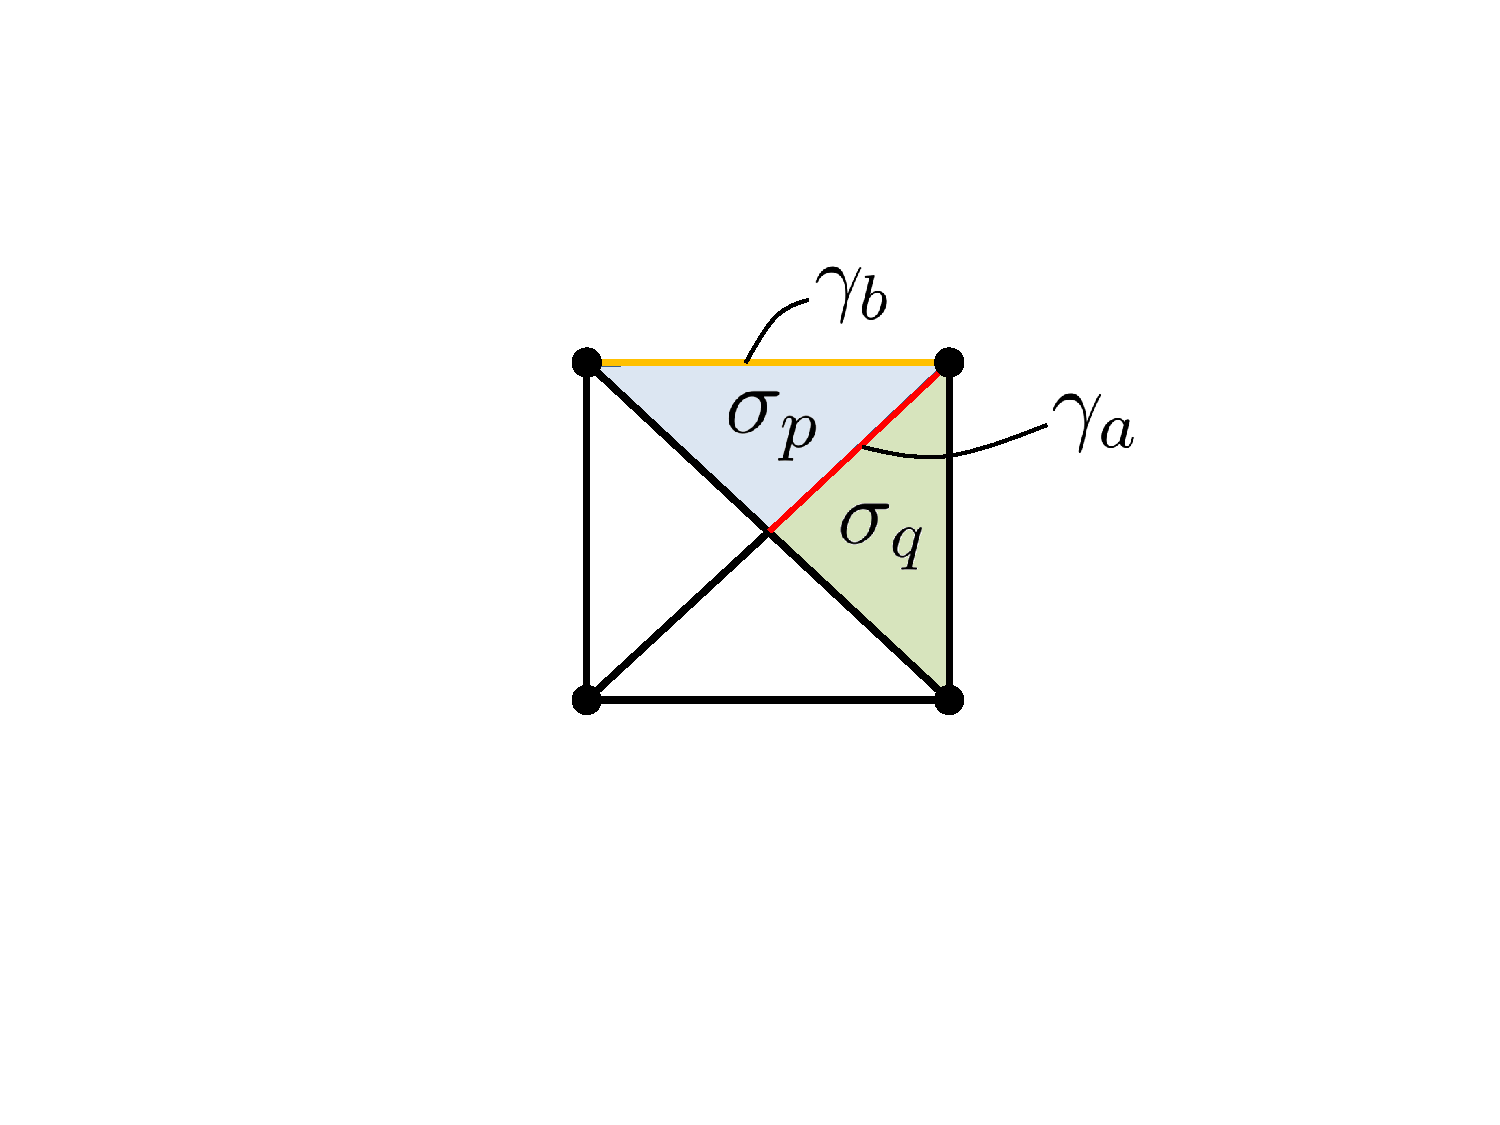
\includegraphics[width = 2.8in,trim=170 190 170 120,clip=true]{facetMinImage.pdf}
	\caption{A representative face of interest.}
	\label{fig:facetMin}
\end{figure}
\begin{center}
\textbf{Face minimization definitions:}
\end{center}
\begin{itemize}
	\item[$\sigma_p$:] A facet on the current face of interest.
	\item[$| \sigma_p |$:] The area of facet $\sigma_p$.
	\item[$c_p$, $\mathbf{g}_p$:] The unknown coefficients that describe the variation of a particular nodal shape function within facet $p$:
	\begin{equation}
		\varphi_p (\mathbf{x}) = c_p + (\mathbf{x} - \mathbf{x}_p) \cdot \mathbf{g}_p
	\end{equation}
	\item[$\mathbf{n}_p$:] The surface normal of facet $p$.
	\item[$\mathbf{x}_p$:] An arbitrarily chosen reference position on facet $p$.
	\item[$\mathcal{L}$:] The set of all ``interior'' segments belonging to the current face.
	\item[$\mathcal{B}$:] The set of all ``boundary'' segments belonging to the current face.
	\item[$\gamma_a$:] An ``interior'' segment, such that $a \in \mathcal{L}$; one that borders two facets: $\sigma_p$ and $\sigma_q$.
	\item[$\gamma_b$:] A ``boundary'' segment, such that $b \in \mathcal{B}$; one that borders a single facet: $\sigma_p$.
	\item[$\bar{c}_b$, $\bar{\mathbf{g}}_b$:] The known coefficients that describe the variation of a particular nodal shape function within segment $b$:
	\begin{equation}
		\varphi_b (\mathbf{x}) = \bar{c}_b + (\mathbf{x} - \mathbf{x}_b) \cdot \bar{\mathbf{g}}_b
	\end{equation}
	\item[$\mathbf{x}_b$:] An arbitrarily chosen reference position on segment $b$.
	\item[$| \gamma_a |$:] The length of segment $\gamma_a$ (similarly for $| \gamma_b |$).
	\item[$\mathbf{P}_a$:] A segment subspace projection operator which maps arbitrary vectors in $\mathbb{R}^3$ to the one-dimensional manifold associated with segment $\gamma_a$. If the tangent space to this manifold is spanned by a single vector $\lambda_a \in \mathbb{R}^3$, then we can determine $\mathbf{P}_a$ via:
	\begin{equation}
		\mathbf{P}_a = \lambda_a \otimes \lambda_a
	\end{equation}
	\item[$\mathbf{P}^{c}_a$:] A complementary subspace projection operator which maps arbitrary vectors in $\mathbb{R}^3$ to the complement of the subspace associated with $\mathbf{P}_a$, obtained via:
	\begin{equation}
		\mathbf{P}^c_a = \mathbf{1} - \mathbf{P}_a
	\end{equation}
	\item[$\varepsilon$:] A scalar-valued measure of the jump in value of a given shape function on interior segments:
	\begin{equation}
		\varepsilon = \varphi_p (\mathbf{x}) - \varphi_q (\mathbf{x})
	\end{equation}
	\begin{equation}
		\varepsilon = c_p + (\mathbf{x} - \mathbf{x}_p) \cdot \mathbf{g}_p - c_q - (\mathbf{x} - \mathbf{x}_q) \cdot \mathbf{g}_q
	\end{equation}
	on boundary segments:
	\begin{equation}
		\varepsilon = \varphi_p (\mathbf{x}) - \varphi_b (\mathbf{x})
	\end{equation}
	\begin{equation}
		\varepsilon = c_p + (\mathbf{x} - \mathbf{x}_p) \cdot \mathbf{g}_p - \bar{c}_b - (\mathbf{x} - \mathbf{x}_b) \cdot \bar{\mathbf{g}}_b
	\end{equation}
	\item[$\Delta$:] A vector-valued measure of the jump in normal derivative of a given shape function, evaluated on an interior segment $\gamma_a$ bordering facets $\sigma_p$ and $\sigma_q$:
	\begin{equation}
		\Delta =\mathbf{P}^c_a ( \nabla \varphi_p (\mathbf{x}) - \nabla \varphi_q (\mathbf{x}) )
	\end{equation}
	\begin{equation}
		\Delta =\mathbf{P}^c_a ( \mathbf{g}_p - \mathbf{g}_q )
	\end{equation}
	\item[$\beta$:] An adjustable parameter, such that $\beta \in (0, 1)$. If $\beta = 0$, $\mathcal{F}$ only penalizes jumps in the normal derivative of the shape function between facets (evaluated on \textit{interior} segments). This effects ``smoothness'' (approaching $C^1$ continuity) of the resulting shape functions. If $\beta = 1$, $\mathcal{F}$ only penalizes jumps in the value of the shape function between facets (evaluated on \textit{interior} segments). This effects $C^0$ continuity of the resulting shape functions (on the interior of the face).
	\item[$\alpha$:] Yet another adjustable parameter such that $\alpha \in (0, 1)$. If $\alpha = 1$, $\mathcal{F}$ will penalize jumps in the value of the shape function between facets and the boundary of the face (evaluated on \textit{boundary} segments). This effects $C^0$ continuity of the resulting shape functions (on the boundary of the face), with no regard for continuity or smoothness across interior segments. If $\alpha = 0$, $\mathcal{F}$ will be expressed only by the relevant $\beta$ terms, meaning there is no penalization to effect continuity with the boundary segments.
	\item[$\mathcal{F}$:] The quadratic functional for a face that is to be minimized with respect to $c_p$ and $\mathbf{g}_p$ for all facets $p$:
	\begin{eqnarray}
	\mathcal{F} = (1-\alpha) \left[ (1-\beta) \sum_{a \in \mathcal{L}} | \gamma_a | \int_{\gamma_a} \frac{1}{2} \Delta \cdot \Delta d \xi + \beta \sum_{a \in \mathcal{L}} \frac{1}{| \gamma_a |} \int_{\gamma_a} \frac{1}{2} \varepsilon^2 d \xi \right] \nonumber \\ + \alpha \sum_{b \in \mathcal{B}} \frac{1}{| \gamma_b |} \int_{\gamma_b} \frac{1}{2} \varepsilon^2 d \xi
\end{eqnarray}
\end{itemize}

\begin{center}
\textbf{Minimization Procedure:}
\end{center}

Now that we have taken care of the relevant definitions, we may elaborate on the minimization procedure. Ultimately, we seek the unknown coefficients $c_p$ and $\mathbf{g}_p$ for all facets $p$ of a given face. These are obtained via
\begin{equation}
	\min_{c_p, \, \mathbf{g}_p} \mathcal{F} \, \, \forall p
\end{equation}
It proves convenient to look at the minimization associated with only one particular interior segment $\gamma_a$:
\begin{equation}
	\mathcal{F}^a = (1-\alpha) \left[ (1-\beta) | \gamma_a | \int_{\gamma_a} \frac{1}{2} \Delta \cdot \Delta d \xi + \beta \frac{1}{| \gamma_a |} \int_{\gamma_a} \frac{1}{2} \varepsilon^2 d \xi \right]
\end{equation}
\begin{equation}
	\frac{\partial \mathcal{F}^a}{\partial c_p} = 0; \qquad \frac{\partial \mathcal{F}^a}{\partial \mathbf{g}_p} = \mathbf{0}
\end{equation}
\begin{equation}
	\frac{\partial \mathcal{F}^a}{\partial c_q} = 0; \qquad \frac{\partial \mathcal{F}^a}{\partial \mathbf{g}_q} = \mathbf{0}
\end{equation}
and one particular boundary segment $\gamma_b$:
\begin{equation}
	\mathcal{F}^b = \alpha \frac{1}{| \gamma_b |} \int_{\gamma_b} \frac{1}{2} \varepsilon^2 d \xi
\end{equation}
\begin{equation}
	\frac{\partial \mathcal{F}^b}{\partial c_p} = 0; \qquad \frac{\partial \mathcal{F}^b}{\partial \mathbf{g}_p} = \mathbf{0}
\end{equation}

For the interior segment:
\begin{equation}
	\frac{\partial \mathcal{F}^a}{\partial c_p} = (1-\alpha) \left[ (1-\beta) | \gamma_a | \int_{\gamma_a} \Delta \cdot \frac{\partial \Delta}{\partial c_p} d \xi + \beta \frac{1}{| \gamma_a |} \int_{\gamma_a} \varepsilon \frac{\partial \varepsilon}{\partial c_p} d \xi \right]
\end{equation}
\begin{equation}
	\frac{\partial \mathcal{F}^a}{\partial \mathbf{g}_p} = (1-\alpha) \left[ (1-\beta) | \gamma_a | \int_{\gamma_a} \Delta \cdot \frac{\partial \Delta}{\partial \mathbf{g}_p} d \xi + \beta \frac{1}{| \gamma_a |} \int_{\gamma_a} \varepsilon \frac{\partial \varepsilon}{\partial \mathbf{g}_p} d \xi \right]
\end{equation}
\begin{equation}
	\frac{\partial \mathcal{F}^a}{\partial c_q} = (1-\alpha) \left[ (1-\beta) | \gamma_a | \int_{\gamma_a} \Delta \cdot \frac{\partial \Delta}{\partial c_q} d \xi + \beta \frac{1}{| \gamma_a |} \int_{\gamma_a} \varepsilon \frac{\partial \varepsilon}{\partial c_q} d \xi \right]
\end{equation}
\begin{equation}
	\frac{\partial \mathcal{F}^a}{\partial \mathbf{g}_q} = (1-\alpha) \left[ (1-\beta) | \gamma_a | \int_{\gamma_a} \Delta \cdot \frac{\partial \Delta}{\partial \mathbf{g}_q} d \xi + \beta \frac{1}{| \gamma_a |} \int_{\gamma_a} \varepsilon \frac{\partial \varepsilon}{\partial \mathbf{g}_q} d \xi \right]
\end{equation}
Examining terms of interest, we find
\begin{equation}
	\frac{\partial \Delta}{\partial c_p} = \frac{\partial \Delta}{\partial c_q} = 0
\end{equation}
\begin{equation}
	\frac{\partial \varepsilon}{\partial c_p} = - \frac{\partial \varepsilon}{\partial c_q} = 1
\end{equation}
\begin{equation}
	\frac{\partial \Delta}{\partial \mathbf{g}_p} = - \frac{\partial \Delta}{\partial \mathbf{g}_q} = \mathbf{P}^c_a
\end{equation}
\begin{equation}
	\frac{\partial \varepsilon}{\partial \mathbf{g}_p} = (\mathbf{x} - \mathbf{x}_p), \quad \frac{\partial \varepsilon}{\partial \mathbf{g}_q} = -(\mathbf{x} - \mathbf{x}_q)
\end{equation}
Making the appropriate substitutions,
\begin{equation}
	\frac{\partial \mathcal{F}^a}{\partial c_p} = (1-\alpha) \left[ \beta \frac{1}{| \gamma_a |} \int_{\gamma_a} \left[ c_p + (\mathbf{x} - \mathbf{x}_p) \cdot \mathbf{g}_p - c_q - (\mathbf{x} - \mathbf{x}_q) \cdot \mathbf{g}_q \right] d \xi \right]
\end{equation}
\begin{equation}
	\frac{\partial \mathcal{F}^a}{\partial c_q} = (1-\alpha) \left[ \beta \frac{1}{| \gamma_a |} \int_{\gamma_a} \left[ -c_p - (\mathbf{x} - \mathbf{x}_p) \cdot \mathbf{g}_p + c_q + (\mathbf{x} - \mathbf{x}_q) \cdot \mathbf{g}_q \right] d \xi \right]
\end{equation}
\begin{eqnarray}
	\frac{\partial \mathcal{F}^a}{\partial \mathbf{g}_p} = (1-\alpha) \left[ (1-\beta) | \gamma_a | \int_{\gamma_a} \mathbf{P}^c_a (\mathbf{g}_p - \mathbf{g}_q ) \, d \xi \right. \nonumber \\ + \left. \beta \frac{1}{| \gamma_a |} \int_{\gamma_a} \left[ c_p + (\mathbf{x} - \mathbf{x}_p) \cdot \mathbf{g}_p - c_q - (\mathbf{x} - \mathbf{x}_q) \cdot \mathbf{g}_q \right] (\mathbf{x} - \mathbf{x}_p) \, d \xi \right]
\end{eqnarray}
\begin{eqnarray}
	\frac{\partial \mathcal{F}^a}{\partial \mathbf{g}_q} = (1-\alpha) \left[ (1-\beta) | \gamma_a | \int_{\gamma_a} \mathbf{P}^c_a (- \mathbf{g}_p + \mathbf{g}_q ) \, d \xi \right. \nonumber \\ + \left. \beta \frac{1}{| \gamma_a |} \int_{\gamma_a} \left[ -c_p - (\mathbf{x} - \mathbf{x}_p) \cdot \mathbf{g}_p + c_q + (\mathbf{x} - \mathbf{x}_q) \cdot \mathbf{g}_q \right] (\mathbf{x} - \mathbf{x}_q) d \xi \right]
\end{eqnarray}
If we define the following terms:
\begin{equation}
	k_{cc} = (1-\alpha) \beta \frac{1}{| \gamma_a |} \int_{\gamma_a} d \xi \quad (1 \times 1)
\end{equation}
\begin{equation}
	\mathbf{k}_{cg}^{(q)} = (1-\alpha) \beta \frac{1}{| \gamma_a |} \int_{\gamma_a} (\mathbf{x} - \mathbf{x}_q) \, d \xi \quad (1 \times 3)
\end{equation}
\begin{equation}
	\mathbf{k}_{gc}^{(p)} = (1-\alpha) \beta \frac{1}{| \gamma_a |} \int_{\gamma_a} (\mathbf{x} - \mathbf{x}_p) d \xi \quad (3 \times 1)
\end{equation}
\begin{eqnarray}
	\mathbf{k}_{gg}^{(p,q)} = (1-\alpha) \left[ \beta \frac{1}{| \gamma_a |} \int_{\gamma_a} (\mathbf{x} - \mathbf{x}_p) \otimes (\mathbf{x} - \mathbf{x}_q) \, d \xi + (1-\beta) | \gamma_a | \int_{\gamma_a} \mathbf{P}^c_a \, d \xi \right] \quad (3 \times 3)
\end{eqnarray}
and if we further define:
\begin{equation}
	\mathbf{K}_{pq}^{(a)} = \left[ \begin{array}{cc} k_{cc} & \mathbf{k}_{cg}^{(q)} \\ \mathbf{k}_{gc}^{(p)} & \mathbf{k}_{gg}^{(p,q)} \end{array} \right] \quad (4 \times 4)
\end{equation}
\begin{equation}
	\mathbf{u}_p = \left\{ \begin{array}{c} c_p \\ \mathbf{g}_p \end{array} \right\} \quad (4 \times 1)
\end{equation}
then we may recast the local minimization for segment $a$ in the form of a local $8\times8$ contribution to the global minimization problem:
\begin{equation}
	\left[ \begin{array}{cc} \mathbf{K}_{pp}^{(a)} & -\mathbf{K}_{pq}^{(a)} \\ -\mathbf{K}_{qp}^{(a)} & \mathbf{K}_{qq}^{(a)} \end{array} \right] \left\{ \begin{array}{c} \mathbf{u}_p \\ \mathbf{u}_q \end{array} \right\} = \left\{ \begin{array}{c} \mathbf{0} \\ \mathbf{0} \end{array} \right\}
\end{equation}

We may proceed in a similar manner to determine a local contribution from the boundary segment:
\begin{equation}
	\frac{\partial \mathcal{F}^b}{\partial c_p} = \alpha \frac{1}{| \gamma_b |} \int_{\gamma_b} \varepsilon \frac{\partial \varepsilon}{\partial c_p} d \xi
\end{equation}
\begin{equation}
	\frac{\partial \mathcal{F}^b}{\partial \mathbf{g}_p} = \alpha \frac{1}{| \gamma_b |} \int_{\gamma_b} \varepsilon \frac{\partial \varepsilon}{\partial \mathbf{g}_p} d \xi
\end{equation}
We recall
\begin{equation}
	\frac{\partial \varepsilon}{\partial c_p} = 1, \quad \frac{\partial \varepsilon}{\partial \mathbf{g}_p} = (\mathbf{x} - \mathbf{x}_p)
\end{equation}
Making the appropriate substitutions,
\begin{equation}
	\frac{\partial \mathcal{F}^b}{\partial c_p} = \alpha \frac{1}{| \gamma_b |} \int_{\gamma_b} \left[ c_p + (\mathbf{x} - \mathbf{x}_p) \cdot \mathbf{g}_p - \bar{c}_b - (\mathbf{x} - \mathbf{x}_b) \cdot \bar{\mathbf{g}}_b \right] d \xi
\end{equation}
\begin{eqnarray}
	\frac{\partial \mathcal{F}^b}{\partial \mathbf{g}_p} = \alpha \frac{1}{| \gamma_b |} \int_{\gamma_b} \left[ c_p + (\mathbf{x} - \mathbf{x}_p) \cdot \mathbf{g}_p - \bar{c}_b - (\mathbf{x} - \mathbf{x}_b) \cdot \bar{\mathbf{g}}_b \right] (\mathbf{x} - \mathbf{x}_p) d \xi
\end{eqnarray}
If we define the following terms:
\begin{equation}
	\bar{k}_{cc} = \alpha \frac{1}{| \gamma_b |} \int_{\gamma_b} d \xi \quad (1 \times 1)
\end{equation}
\begin{equation}
	\bar{\mathbf{k}}_{cg}^{(b)} = \alpha \frac{1}{| \gamma_b |} \int_{\gamma_b} (\mathbf{x} - \mathbf{x}_b) d \xi \quad (1 \times 3)
\end{equation}
\begin{equation}
	\bar{\mathbf{k}}_{gc}^{(p)} = \alpha \frac{1}{| \gamma_b |} \int_{\gamma_b} (\mathbf{x} - \mathbf{x}_p) d \xi \quad (3 \times 1)
\end{equation}
\begin{eqnarray}
	\bar{\mathbf{k}}_{gg}^{(p,b)} = \alpha \frac{1}{| \gamma_b |} \int_{\gamma_b} (\mathbf{x} - \mathbf{x}_p) \otimes (\mathbf{x} - \mathbf{x}_b) d \xi \quad (3 \times 3)
\end{eqnarray}
and if we further define:
\begin{equation}
	\bar{\mathbf{K}}_{pb}^{(b)} = \left[ \begin{array}{cc} \bar{k}_{cc} & \bar{\mathbf{k}}_{cg}^{(b)} \\ \bar{\mathbf{k}}_{gc}^{(p)} & \bar{\mathbf{k}}_{gg}^{(p,b)} \end{array} \right] \quad (4 \times 4)
\end{equation}
\begin{equation}
	\bar{\mathbf{u}}_b = \left\{ \begin{array}{c} \bar{c}_b \\ \bar{\mathbf{g}}_b \end{array} \right\} \quad (4 \times 1)
\end{equation}
then we may recast the local minimization for segment $b$ in the form of local $4\times4$ contributions to the global minimization problem:
\begin{equation}
	\bar{\mathbf{K}}_{pp}^{(b)} \mathbf{u}_p = \bar{\mathbf{K}}_{pb}^{(b)} \bar{\mathbf{u}}_b
\end{equation}

\newpage

\begin{center}
\textbf{Integration of Polynomial Expressions on Arbitrary Polytopes:}
\end{center}

Suppose we wish to integrate a polynomial expression $P^{(p)}(\mathbf{x})$ of degree $p$
\begin{equation}
	P^{(p)}(\mathbf{x}) = \sum_{r=0}^{p} a_r \mathbf{x}^{\otimes r}
\end{equation}
over an arbitrary closed $n$-polytope $\Omega_q \subset \mathcal{V}$ ($\mathcal{V}$ being an isometry of $\mathbb{R}^n$), which itself is embedded in $\mathbb{R}^d$ (such that $\mathbf{x} \in \mathbb{R}^d$). We identify $\mathbf{x}^{\otimes r}$ as a tensor of rank $r$ (e.g. $\mathbf{x}^{\otimes 2} = \mathbf{x} \otimes \mathbf{x}$). We are interested in computing
\begin{equation}
	\int_{\Omega_q} P^{(p)}(\mathbf{x}) d \Omega = \sum_{r=0}^{p} a_r \int_{\Omega_q} \mathbf{x}^{\otimes r} d \Omega,
\end{equation}
meaning we must be able to integrate $\int_{\Omega_q} \mathbf{x}^{\otimes r} d \Omega \, \, \forall r$. Let us suppose that $\mathbf{x}$ may be written as $\mathbf{x} = \mathbf{x}_q + \hat{\mathbf{x}}$, where $\mathbf{x}_q \in \mathbb{R}^d$ is some fixed reference position on the $n$-polytope, and $\hat{\mathbf{x}} \in \mathcal{V}$ is variable. Thus,
\begin{equation}
	\int_{\Omega_q} \mathbf{x}^{\otimes r} d \Omega = \int_{\Omega_q} (\mathbf{x}_q + \hat{\mathbf{x}})^{\otimes r} d \Omega = \sum_{k = 0}^r \binom{r}{k} \, \mbox{Sym}
\bigg( \mathbf{x}_q^{\otimes (r-k)} \otimes \int_{\Omega_q} \hat{\mathbf{x}}^{\otimes k} d \Omega \bigg) ,
\end{equation}
where $\mbox{Sym} ( \mathbf{T} )$ denotes the symmetric part of tensor $\mathbf{T}$. By the divergence theorem
\begin{equation}
	\int_{\Omega_q} \hat{\mathbf{x}}^{\otimes k} d \Omega = \frac{1}{n+k} \int_{\Gamma} \langle \hat{\mathbf{x}}^{\otimes (k+1)} , \mathbf{n} \rangle \, d \Gamma
\end{equation}
where $\Gamma$ constitutes the boundary of $\Omega_q$, and $\mathbf{n} \in V$ is the unit outward normal to $\Omega_q$. If we suppose that $\Gamma = \cup_{\alpha} \Gamma_{\alpha}$, where $\Gamma_{\alpha} \subset \mathcal{S}_{\alpha}$ ($\mathcal{S}_\alpha$ being an isometry of $\mathbb{R}^{(n-1)}$) are $(n-1)$-polytopes, then we have
\begin{equation}
	\int_{\Omega_q} \hat{\mathbf{x}}^{\otimes k} d \Omega = \frac{1}{n+k} \sum_{\alpha} \mathbf{x}_{\alpha} \cdot \mathbf{n}_{\alpha} \int_{\Gamma_{\alpha}} \hat{\mathbf{x}}^{\otimes k}   d \Gamma
\end{equation}
where we suppose $\hat{\mathbf{x}} = \mathbf{x}_{\alpha} + \hat{\mathbf{x}}_{\alpha}$, $\mathbf{x}_{\alpha} \in \mathcal{V}$ is again some fixed reference position on the $(n-1)$-polytope of interest, and $\hat{\mathbf{x}}_{\alpha} \in \mathcal{S}_{\alpha}$ is variable. Therefore,
\begin{equation}
	\int_{\Omega_q} \mathbf{x}^{\otimes r} d \Omega = \sum_{k = 0}^r \binom{r}{k} \frac{1}{n+k} \, \mbox{Sym} \bigg( \mathbf{x}_q^{\otimes (r-k)} \otimes \sum_{\alpha} \mathbf{x}_{\alpha} \cdot \mathbf{n}_{\alpha} \int_{\Gamma_{\alpha}} \hat{\mathbf{x}}^{\otimes k}   d \Gamma \bigg) .
\end{equation}
Note that
\begin{equation}
	\mathbf{x}_{\alpha} \cdot \mathbf{n}_{\alpha} = (\mathbf{x} - \mathbf{x}_q - \hat{\mathbf{x}}_{\alpha}) \cdot \mathbf{n}_{\alpha} = (\mathbf{x} - \mathbf{x}_q) \cdot \mathbf{n}_{\alpha} =  (\mathbf{a}_{\alpha} - \mathbf{x}_q) \cdot \mathbf{n}_{\alpha}
\end{equation}
\begin{equation}
	\hat{\mathbf{x}} = (\mathbf{x} - \mathbf{x}_q)
\end{equation}
where $\mathbf{x} = \mathbf{a}_{\alpha} + \hat{\mathbf{a}}_{\alpha}$ is yet another shifted coordinate system with $\hat{\mathbf{a}}_{\alpha} \in \mathcal{S}_{\alpha}$, and $\mathbf{a}_{\alpha} \in \mathbb{R}^d$ a fixed reference position on the $(n-1)$-polytope denoted by $\alpha$. Consequently,
\begin{equation}
	\int_{\Omega_q} \mathbf{x}^{\otimes r} d \Omega = \sum_{k = 0}^r \binom{r}{k} \frac{1}{n+k} \, \mbox{Sym} \bigg( \mathbf{x}_q^{\otimes (r-k)} \otimes \sum_{\alpha} (\mathbf{a}_{\alpha} - \mathbf{x}_q) \cdot \mathbf{n}_{\alpha} \int_{\Gamma_{\alpha}} (\mathbf{x} - \mathbf{x}_q)^{\otimes k} d \Gamma \bigg) .
\end{equation}
Observing that
\begin{equation}
	\int_{\Gamma_{\alpha}} (\mathbf{x} - \mathbf{x}_q)^{\otimes k} d \Gamma = \sum_{j = 0}^k \binom{k}{j} (-1)^{(k-j)} \, \mbox{Sym} \bigg( \mathbf{x}_q^{\otimes (k-j)} \otimes \int_{\Gamma_{\alpha}} \mathbf{x}^{\otimes j} d \Gamma \bigg)
\end{equation}
we arrive at
\begin{equation}
	\int_{\Omega_q} \mathbf{x}^{\otimes r} d \Omega = \sum_{k = 0}^r \sum_{j = 0}^k \binom{r}{k} \binom{k}{j} \frac{(-1)^{(k-j)}}{n+k} \, \mbox{Sym} \bigg( \mathbf{x}_q^{\otimes (r-j)} \otimes \sum_{\alpha} (\mathbf{a}_{\alpha} - \mathbf{x}_q) \cdot \mathbf{n}_{\alpha} \int_{\Gamma_{\alpha}} \mathbf{x}^{\otimes j} d \Gamma \bigg) .
\end{equation}
It remains to be shown (by induction) that the following simplified expression holds:
\begin{equation}
	\int_{\Omega_q} \mathbf{x}^{\otimes r} d \Omega = \frac{1}{n+r} \left[ r \, \mbox{Sym} \bigg( \mathbf{x}_q \otimes \int_{\Omega_q} \mathbf{x}^{\otimes (r-1)} d \Omega \bigg) + \sum_{\alpha} (\mathbf{a}_{\alpha} - \mathbf{x}_q) \cdot \mathbf{n}_{\alpha} \int_{\Gamma_{\alpha}} \mathbf{x}^{\otimes r} d \Gamma \right] .
\end{equation}

Consider now a two-noded segment $\gamma$ whose nodal coordinates are given by $\mathbf{a}_1, \, \mathbf{a}_2 \in \mathbb{R}^3$. The integral evaluations (up to $r = 4$) on the segment reduce to:
\begin{equation}
	\int_{\gamma} \, d \gamma \equiv | \gamma | = || \mathbf{a}_{2} - \mathbf{a}_{1} ||_2
\end{equation}
\begin{equation}
	\int_{\gamma} \mathbf{x} \, d \gamma = \frac{| \gamma |}{2} (\mathbf{a}_{1} + \mathbf{a}_{2})
\end{equation}
\begin{equation}
	\int_{\gamma} \mathbf{x}^{\otimes 2} \, d \gamma = \frac{| \gamma |}{3} \left[ \mbox{Sym} \bigg( \mathbf{a}_1 \otimes \mathbf{a}_{2} \bigg) + \mathbf{a}_1^{\otimes 2} + \mathbf{a}_2^{\otimes 2} \right]
\end{equation}
\begin{equation}
	\int_{\gamma} \mathbf{x}^{\otimes 3} \, d \gamma = \frac{| \gamma |}{4} \left[ \mbox{Sym} \bigg( \mathbf{a}_1^{\otimes 2} \otimes \mathbf{a}_{2} + \mathbf{a}_1 \otimes \mathbf{a}_2^{\otimes 2} \bigg) + \mathbf{a}_1^{\otimes 3} + \mathbf{a}_2^{\otimes 3} \right]
\end{equation}
\begin{equation}
	\int_{\gamma} \mathbf{x}^{\otimes 4} \, d \gamma = \frac{| \gamma |}{5} \left[ \mbox{Sym} \bigg( \mathbf{a}_1^{\otimes 3} \otimes \mathbf{a}_{2} + \mathbf{a}_1^{\otimes 2} \otimes \mathbf{a}_2^{\otimes 2} + \mathbf{a}_1 \otimes \mathbf{a}_2^{\otimes 3} \bigg) + \mathbf{a}_1^{\otimes 4} + \mathbf{a}_2^{\otimes 4} \right]
\end{equation}

Considering an $m$-noded facet $\sigma$ whose nodal coordinates (listed in cyclic order around the facet) are given by $\mathbf{b}_j \in \mathbb{R}^3$ ($j = 1, \, \ldots, \, m$), the integral evaluations on the facet reduce to:
\begin{equation}
	\mathbf{A} = \frac{1}{2} \sum_{j = 2}^{m-1} (\mathbf{b}_{j} - \mathbf{b}_1) \times (\mathbf{b}_{j+1} - \mathbf{b}_{1})
\end{equation}
\begin{equation}
	\int_{\sigma} \, d \sigma \equiv | \sigma | = || \mathbf{A} ||_2
\end{equation}
\begin{equation}
	\mathbf{N} = \frac{\mathbf{A}}{| \sigma |}
\end{equation}
\begin{eqnarray}
	\int_{\sigma} \mathbf{x}^{\otimes r} d \sigma = \frac{1}{2+r} \left[ r \, \mbox{Sym} \bigg( \mathbf{b}_1 \otimes \int_{\sigma} \mathbf{x}^{\otimes (r-1)} \, d \sigma \bigg) \qquad \qquad \qquad \qquad \right. \nonumber \\ + \left. \sum_{j = 2}^{m-1} \bigg( \mathbf{N} \cdot \left[ (\mathbf{b}_{j} - \mathbf{b}_1) \times (\mathbf{b}_{j+1} - \mathbf{b}_{1}) \right] \bigg) \frac{1}{| \gamma_j |}\int_{\gamma_j} \mathbf{x}^{\otimes r} \, d \gamma \right] .
\end{eqnarray}

For an $f$-faceted cell $\omega$ whose facets (specified in no particular order) are denoted by $\sigma_\alpha$ ($\alpha = 1, \, \ldots, \, f$), the volume of the cell $|\omega|$ is computed as:
\begin{equation}
	\int_{\omega} \, d \omega \equiv | \omega | = \frac{1}{3} \sum_{\alpha=1}^f \mathbf{x}_{\alpha} \cdot (z_\alpha \mathbf{n}_{\alpha}) | \sigma_{\alpha} |
\end{equation}
where $\mathbf{x}_\alpha$ is an arbitrary reference position on facet $\sigma_\alpha$, $\mathbf{n}_\alpha$ is the facet's surface normal (not necessarily outward facing with respect to the cell in question), and $z_\alpha = \pm 1$ is a facet ``orientation consistency'' factor (ensuring that all cell facet normals are consistent with an all-outward orientation). In practice the $z_\alpha$ factors could either be specified directly, or they could be determined algorithmically based on the facet node numberings. Higher-order moments for the cell may be computed via:
\begin{equation}
	\int_{\omega} \mathbf{x}^{\otimes r} \, d \omega = \frac{1}{3+r} \sum_{\alpha=1}^f \mathbf{x}_{\alpha} \cdot (z_\alpha \mathbf{n}_{\alpha}) \int_{\sigma_{\alpha}} \mathbf{x}^{\otimes r} \, d \sigma .
\end{equation}

\newpage

\begin{center}
\textbf{Quadrature Consistency:}
\end{center}

Consider the strong-form of equilibrium in the abscence of body force:
\begin{equation}
	T_{ij,j} = 0 \quad \forall x_i \in B,
\end{equation}
the equivalent weak-form of equilibirum in the abscence of body force:
\begin{equation}
	\int_{\Omega} T_{ij,j} dv = \int_{\Gamma} t_i da \quad \forall \Omega \subset B
\end{equation}
and the Galerkin approximation to the weak form:
\begin{equation}
	\int_{\Omega} T_{ij} \varphi_{a,j} dv = \int_{\Gamma} t_i \varphi_a da = \int_{\Gamma} T_{ij} \varphi_a n_j da \quad \forall a.
\end{equation}
Technically speaking, this last may only hold on element domains, i.e.
\begin{equation}
	\int_{\Omega_e} T_{ij} \varphi_{a,j} dv = \int_{\Gamma_e} T_{ij} \varphi_a n_j da \quad \forall a.
\end{equation}
Let us suppose that the stress field satisfies a linear spatial variation (corresponding to a quadratic displacement field for a linear elastic material), namely
\begin{equation}
	T_{ij} (x_k) = \bar{T}_{ij} + \bar{T}_{ij,k} x_k,
\end{equation}
such that
\begin{equation}
	\int_{\Omega_e} (\bar{T}_{ij} + \bar{T}_{ij,k} x_k) \varphi_{a,j} dv = \int_{\Gamma_e} (\bar{T}_{ij} + \bar{T}_{ij,k} x_k) \varphi_a n_j da \quad \forall a.
\end{equation}
This implies that
\begin{equation}
	\bar{T}_{ij} \bigg(\int_{\Omega_e} \varphi_{a,j} dv - \int_{\Gamma_e} \varphi_a n_j da \bigg) + \bar{T}_{ij,k} \bigg( \int_{\Omega_e} x_k \varphi_{a,j} dv - \int_{\Gamma_e} x_k \varphi_a n_j da \bigg) = 0  \quad \forall a.
\end{equation}
However, since the displacement field is arbitrary, $\bar{T}_{ij}$ and $\bar{T}_{ij,k}$ are therefore arbitrary, and we require
\begin{equation}
	\int_{\Omega_e} \varphi_{a,j} dv = \int_{\Gamma_e} \varphi_a n_j da \quad \forall a,
\end{equation}
\begin{equation}
	\int_{\Omega_e} x_k \varphi_{a,j} dv = \int_{\Gamma_e} x_k \varphi_a n_j da \quad \forall a.
\end{equation}
These conditions constitute first- and second-order ``quadrature consistency,'' respectively. For PEM elements, this amounts to
\begin{equation}
	\sum_{q} | \omega_q | \bar{\varphi}_{a,j}^{(q)} = \sum_{\alpha} | \sigma_{\alpha} | n_j^{(\alpha)} \bar{\varphi}_a^{(\alpha)},
\end{equation}
\begin{equation}
	\sum_{q} | \omega_q | \bar{x}_k^{(q)} \bar{\varphi}_{a,j}^{(q)} = \sum_{\alpha} | \sigma_{\alpha} | \bar{x}_k^{(\alpha)} n_j^{(\alpha)} \bar{\varphi}_a^{(\alpha)}.
\end{equation}
This suggests that even if the displacement field itself is not able to exactly reproduce a spatially quadratic field (due to interpolation error), second-order quadrature consistency may still guarantee exact integration of the weak form when the \textit{nodes} are set consistent with such a field. It may well be the case that such elements will exhibit improved convergence in the $H^1$ energy semi-norm, but will otherwise retain second-order convergence in the $L^2$ displacement norm. Improvement in the $L^2$ convergence rate may perhaps be had by further refinement of the element into a greater number of quadrature sub-cells.

``Quadrature consistency'' simply asserts that we must be able to evaluate weak form integrals exactly using the element's quadrature rule.  we may suppose that the stress field assumes the following (more general) form:
\begin{equation}
	T_{ij} (x_k) = \sum_b c_b f^{(b)}_{ij} ( x_k )
\end{equation}
where $f^{(a)}_{ij}$ are a set of independent spatially varying functions. In this context,
\begin{equation}
	\int_{\Omega_e} \bigg( \sum_b c_b f^{(b)}_{ij} ( x_k ) \bigg) \varphi_{a,j} dv = \int_{\Gamma_e} \bigg( \sum_b c_b f^{(b)}_{ij} ( x_k ) \bigg) \varphi_a n_j da \quad \forall a
\end{equation}
\begin{equation}
	\sum_b c_b \bigg( \int_{\Omega_e} f^{(b)}_{ij} ( x_k ) \varphi_{a,j} dv - \int_{\Gamma_e} f^{(b)}_{ij} ( x_k ) \varphi_a n_j da \bigg) = 0 \quad \forall i, \, a
\end{equation}
\begin{equation}
	\int_{\Omega_e} f^{(b)}_{ij} ( x_k ) \varphi_{a,j} dv = \int_{\Gamma_e} f^{(b)}_{ij} ( x_k ) \varphi_a n_j da \quad \forall i, \, a, \, b
\end{equation}

We further suppose that quadrature consistency may yet need to hold for both faces and edges. In the case of a face, we postulate that a kind of ``weak'' Stokes' theorem hold for the face interpolants. Likewise, the edges may need to satisfy the divergence theorem.

\newpage

\begin{center}
\textbf{Quadratically Complete PEM Elements:}
\end{center}

Let us consider the consequences of allowing for the shape functions to vary quadratically within each quadrature cell, i.e.
\begin{equation}
	\varphi_p (\mathbf{x}) = c_p + (\mathbf{x} - \mathbf{x}_p) \cdot \mathbf{g}_p + (\mathbf{x} - \mathbf{x}_p) \otimes (\mathbf{x} - \mathbf{x}_p) \colon \mathbf{H}_p,
\end{equation}
where $\mathbf{H}_p$ is a symmetric rank-2 tensor. Notably
\begin{equation}
	\varepsilon = c_p + (\mathbf{x} - \mathbf{x}_p) \cdot \mathbf{g}_p + (\mathbf{x} - \mathbf{x}_p) \otimes (\mathbf{x} - \mathbf{x}_p) \colon \mathbf{H}_p - c_q - (\mathbf{x} - \mathbf{x}_q) \cdot \mathbf{g}_q - (\mathbf{x} - \mathbf{x}_q) \otimes (\mathbf{x} - \mathbf{x}_q) \colon \mathbf{H}_q
\end{equation}
\begin{equation}
	\Delta = \mathbf{P}^c_a \left\{ \mathbf{g}_p + 2 \mathbf{H}_p (\mathbf{x} - \mathbf{x}_p) - \mathbf{g}_q - 2 \mathbf{H}_q (\mathbf{x} - \mathbf{x}_q) \right\}.
\end{equation}
We further define $\theta$ as a tensor-valued measure of the jump in normal second derivative:
\begin{equation}
	\theta = \mathbf{P}^c_a \left\{ 2\mathbf{H}_p - 2 \mathbf{H}_q \right\} .
\end{equation}
The proposed quadratic functional for the element's cell minimization procedure will take the form
\begin{eqnarray}
	\mathcal{F} = (1-\alpha) \left[ (1 - \gamma) \bigg( (1-\beta) \sum_{a \in \mathcal{L}} | \sigma_a | \int_{\sigma_a} \frac{1}{2} \Delta \cdot \Delta d \sigma + \beta \sum_{a \in \mathcal{L}} \frac{1}{| \sigma_a |} \int_{\sigma_a} \frac{1}{2} \varepsilon^2 d \sigma \bigg) \right. \nonumber \\ + \left. \gamma \sum_{a \in \mathcal{L}} | \sigma_a |^3 \int_{\sigma_a} \frac{1}{2} \theta \colon \theta d \sigma \right] \nonumber \\ + \alpha \sum_{b \in \mathcal{B}} \frac{1}{| \sigma_b |} \int_{\sigma_b} \frac{1}{2} \varepsilon^2 d \sigma.
\end{eqnarray}
Note that this functional includes an additional penalization of $\theta$ (via a parameter $\gamma \in (0, \, 1)$) that -- to coin a phrase -- ``hates wiggles.'' We may proceed in minimizing $\mathcal{F}$ via:
\begin{equation}
	\min_{c_p, \, \mathbf{g}_p, \, \mathbf{H}_p} \mathcal{F} \, \, \forall p
\end{equation}
Revisiting our earlier derivation, it proves convenient to look at the minimization associated with only one particular interior facet $\sigma_a$:
\begin{equation}
	\mathcal{F}^a = (1-\alpha) \left[ (1-\gamma) \bigg( (1-\beta) | \sigma_a | \int_{\sigma_a} \frac{1}{2} \Delta \cdot \Delta d \sigma + \beta \frac{1}{| \sigma_a |} \int_{\sigma_a} \frac{1}{2} \varepsilon^2 d \sigma \bigg) + \gamma | \sigma_a |^3 \int_{\sigma_a} \frac{1}{2} \theta \colon \theta d \sigma \right]
\end{equation}
\begin{equation}
	\frac{\partial \mathcal{F}^a}{\partial c_p} = 0; \qquad \frac{\partial \mathcal{F}^a}{\partial \mathbf{g}_p} = \mathbf{0}; \qquad \frac{\partial \mathcal{F}^a}{\partial \mathbf{H}_p} = \mathbf{0}
\end{equation}
\begin{equation}
	\frac{\partial \mathcal{F}^a}{\partial c_q} = 0; \qquad \frac{\partial \mathcal{F}^a}{\partial \mathbf{g}_q} = \mathbf{0}; \qquad \frac{\partial \mathcal{F}^a}{\partial \mathbf{H}_q} = \mathbf{0}
\end{equation}
and one particular exterior boundary $\sigma_b$:
\begin{equation}
	\mathcal{F}^b = \alpha \frac{1}{| \sigma_b |} \int_{\sigma_b} \frac{1}{2} \varepsilon^2 d \sigma
\end{equation}
\begin{equation}
	\frac{\partial \mathcal{F}^b}{\partial c_p} = 0; \qquad \frac{\partial \mathcal{F}^b}{\partial \mathbf{g}_p} = \mathbf{0}; \qquad \frac{\partial \mathcal{F}^b}{\partial \mathbf{H}_p} = \mathbf{0}
\end{equation}

For an interior facet:
\begin{eqnarray}
	\frac{\partial \mathcal{F}^a}{\partial c_p} = (1-\alpha) \left[ (1-\gamma) \bigg( (1-\beta) | \sigma_a | \int_{\sigma_a} \Delta \cdot \frac{\partial \Delta}{\partial c_p} d \sigma + \beta \frac{1}{| \sigma_a |} \int_{\sigma_a} \varepsilon \frac{\partial \varepsilon}{\partial c_p} d \sigma \bigg) \right. \nonumber \\ \left. + \gamma | \sigma_a |^3 \int_{\sigma_a} \frac{1}{2} \theta \colon \frac{\partial \theta}{\partial c_p} d \sigma \right]
\end{eqnarray}
\begin{eqnarray}
	\frac{\partial \mathcal{F}^a}{\partial \mathbf{g}_p} = (1-\alpha) \left[ (1-\gamma) \bigg( (1-\beta) | \sigma_a | \int_{\sigma_a} \Delta \cdot \frac{\partial \Delta}{\partial \mathbf{g}_p} d \sigma + \beta \frac{1}{| \sigma_a |} \int_{\sigma_a} \varepsilon \frac{\partial \varepsilon}{\partial \mathbf{g}_p} d \sigma \bigg) \right. \nonumber \\ \left. + \gamma | \sigma_a |^3 \int_{\sigma_a} \frac{1}{2} \theta \colon \frac{\partial \theta}{\partial \mathbf{g}_p} d \sigma \right]
\end{eqnarray}
\begin{eqnarray}
	\frac{\partial \mathcal{F}^a}{\partial \mathbf{H}_p} = (1-\alpha) \left[ (1-\gamma) \bigg( (1-\beta) | \sigma_a | \int_{\sigma_a} \Delta \cdot \frac{\partial \Delta}{\partial \mathbf{H}_p} d \sigma + \beta \frac{1}{| \sigma_a |} \int_{\sigma_a} \varepsilon \frac{\partial \varepsilon}{\partial \mathbf{H}_p} d \sigma \bigg) \right. \nonumber \\ \left. + \gamma | \sigma_a |^3 \int_{\sigma_a} \frac{1}{2} \theta \colon \frac{\partial \theta}{\partial \mathbf{H}_p} d \sigma \right]
\end{eqnarray}
\begin{eqnarray}
	\frac{\partial \mathcal{F}^a}{\partial c_q} = (1-\alpha) \left[ (1-\gamma) \bigg( (1-\beta) | \sigma_a | \int_{\sigma_a} \Delta \cdot \frac{\partial \Delta}{\partial c_q} d \sigma + \beta \frac{1}{| \sigma_a |} \int_{\sigma_a} \varepsilon \frac{\partial \varepsilon}{\partial c_q} d \sigma \bigg) \right. \nonumber \\ \left. + \gamma | \sigma_a |^3 \int_{\sigma_a} \frac{1}{2} \theta \colon \frac{\partial \theta}{\partial c_q} d \sigma \right]
\end{eqnarray}
\begin{eqnarray}
	\frac{\partial \mathcal{F}^a}{\partial \mathbf{g}_q} = (1-\alpha) \left[ (1-\gamma) \bigg( (1-\beta) | \sigma_a | \int_{\sigma_a} \Delta \cdot \frac{\partial \Delta}{\partial \mathbf{g}_q} d \sigma + \beta \frac{1}{| \sigma_a |} \int_{\sigma_a} \varepsilon \frac{\partial \varepsilon}{\partial \mathbf{g}_q} d \sigma \bigg) \right. \nonumber \\ \left. + \gamma | \sigma_a |^3 \int_{\sigma_a} \frac{1}{2} \theta \colon \frac{\partial \theta}{\partial \mathbf{g}_q} d \sigma \right]
\end{eqnarray}
\begin{eqnarray}
	\frac{\partial \mathcal{F}^a}{\partial \mathbf{H}_q} = (1-\alpha) \left[ (1-\gamma) \bigg( (1-\beta) | \sigma_a | \int_{\sigma_a} \Delta \cdot \frac{\partial \Delta}{\partial \mathbf{H}_q} d \sigma + \beta \frac{1}{| \sigma_a |} \int_{\sigma_a} \varepsilon \frac{\partial \varepsilon}{\partial \mathbf{H}_q} d \sigma \bigg) \right. \nonumber \\ \left. + \gamma | \sigma_a |^3 \int_{\sigma_a} \frac{1}{2} \theta \colon \frac{\partial \theta}{\partial \mathbf{H}_q} d \sigma \right]
\end{eqnarray}
Examining terms of interest, we find
\begin{equation}
	\frac{\partial \theta}{\partial c_p} = \frac{\partial \theta}{\partial c_q} = 0
\end{equation}
\begin{equation}
	\frac{\partial \Delta}{\partial c_p} = \frac{\partial \Delta}{\partial c_q} = \mathbf{0}
\end{equation}
\begin{equation}
	\frac{\partial \varepsilon}{\partial c_p} = - \frac{\partial \varepsilon}{\partial c_q} = 1
\end{equation}
\begin{equation}
	\frac{\partial \theta}{\partial \mathbf{g}_p} = \frac{\partial \theta}{\partial \mathbf{g}_q} = \mathbf{0}
\end{equation}
\begin{equation}
	\frac{\partial \Delta}{\partial \mathbf{g}_p} = - \frac{\partial \Delta}{\partial \mathbf{g}_q} = \mathbf{P}^c_a
\end{equation}
\begin{equation}
	\frac{\partial \varepsilon}{\partial \mathbf{g}_p} = (\mathbf{x} - \mathbf{x}_p), \quad \frac{\partial \varepsilon}{\partial \mathbf{g}_q} = -(\mathbf{x} - \mathbf{x}_q)
\end{equation}
\begin{equation}
	\frac{\partial \theta_{kl}}{\partial H_{rs}^{(p)}} = - \frac{\partial \theta_{kl}}{\partial H_{rs}^{(q)}} = P^{(c,a)}_{kr} \delta_{sl} + P^{(c,a)}_{ks} \delta_{rl}
\end{equation}
\begin{equation}
	\frac{\partial \Delta_k}{\partial H_{rs}^{(p)}} = P^{(c,a)}_{kr} (x_s - x^{(p)}_s) + P^{(c,a)}_{ks} (x_r - x^{(p)}_r) 
\end{equation}
\begin{equation}
	\frac{\partial \Delta_k}{\partial H_{rs}^{(q)}} = - P^{(c,a)}_{kr} (x_s - x^{(q)}_s) - P^{(c,a)}_{ks} (x_r - x^{(q)}_r) 
\end{equation}
\begin{equation}
	\frac{\partial \varepsilon}{\partial \mathbf{H}_p} = (\mathbf{x} - \mathbf{x}_p) \otimes (\mathbf{x} - \mathbf{x}_p), \quad \frac{\partial \varepsilon}{\partial \mathbf{H}_q} = -(\mathbf{x} - \mathbf{x}_q) \otimes (\mathbf{x} - \mathbf{x}_q)
\end{equation}
Making the appropriate substitutions,
\begin{eqnarray}
	\frac{\partial \mathcal{F}^a}{\partial c_p} = (1-\alpha) (1-\gamma) \beta \frac{1}{| \sigma_a |} \int_{\sigma_a} \left[ c_p + (\mathbf{x} - \mathbf{x}_p) \cdot \mathbf{g}_p + (\mathbf{x} - \mathbf{x}_p) \otimes (\mathbf{x} - \mathbf{x}_p) \colon \mathbf{H}_p \right. \nonumber \\ \left. - c_q - (\mathbf{x} - \mathbf{x}_q) \cdot \mathbf{g}_q - (\mathbf{x} - \mathbf{x}_q) \otimes (\mathbf{x} - \mathbf{x}_q) \colon \mathbf{H}_q \right] d \sigma
\end{eqnarray}
\begin{eqnarray}
	\frac{\partial \mathcal{F}^a}{\partial c_q} = (1-\alpha) (1-\gamma) \beta \frac{1}{| \sigma_a |} \int_{\sigma_a} \left[ - c_p - (\mathbf{x} - \mathbf{x}_p) \cdot \mathbf{g}_p - (\mathbf{x} - \mathbf{x}_p) \otimes (\mathbf{x} - \mathbf{x}_p) \colon \mathbf{H}_p \right. \nonumber \\ \left. + c_q + (\mathbf{x} - \mathbf{x}_q) \cdot \mathbf{g}_q + (\mathbf{x} - \mathbf{x}_q) \otimes (\mathbf{x} - \mathbf{x}_q) \colon \mathbf{H}_q \right] d \sigma
\end{eqnarray}
\begin{eqnarray}
	\frac{\partial \mathcal{F}^a}{\partial \mathbf{g}_p} = (1-\alpha)(1-\gamma)(1-\beta) | \sigma_a | \int_{\sigma_a} \mathbf{P}^c_a \bigg( \mathbf{g}_p + 2 \mathbf{H}_p (\mathbf{x} - \mathbf{x}_p) - \mathbf{g}_q - 2 \mathbf{H}_q (\mathbf{x} - \mathbf{x}_q) \bigg) \, d \sigma \nonumber \\ + (1-\alpha) (1-\gamma) \beta \frac{1}{| \sigma_a |} \int_{\sigma_a} \left[ c_p + (\mathbf{x} - \mathbf{x}_p) \cdot \mathbf{g}_p + (\mathbf{x} - \mathbf{x}_p) \otimes (\mathbf{x} - \mathbf{x}_p) \colon \mathbf{H}_p \right. \nonumber \\ \left. - c_q - (\mathbf{x} - \mathbf{x}_q) \cdot \mathbf{g}_q - (\mathbf{x} - \mathbf{x}_q) \otimes (\mathbf{x} - \mathbf{x}_q) \colon \mathbf{H}_q \right] (\mathbf{x} - \mathbf{x}_p) \, d \sigma
\end{eqnarray}
\begin{eqnarray}
	\frac{\partial \mathcal{F}^a}{\partial \mathbf{g}_q} = (1-\alpha)(1-\gamma)(1-\beta) | \sigma_a | \int_{\sigma_a} \mathbf{P}^c_a \bigg( - \mathbf{g}_p - 2 \mathbf{H}_p (\mathbf{x} - \mathbf{x}_p) + \mathbf{g}_q + 2 \mathbf{H}_q (\mathbf{x} - \mathbf{x}_q) \bigg) \, d \sigma \nonumber \\ + (1-\alpha) (1-\gamma) \beta \frac{1}{| \sigma_a |} \int_{\sigma_a} \left[ - c_p - (\mathbf{x} - \mathbf{x}_p) \cdot \mathbf{g}_p - (\mathbf{x} - \mathbf{x}_p) \otimes (\mathbf{x} - \mathbf{x}_p) \colon \mathbf{H}_p \right. \nonumber \\ \left. + c_q + (\mathbf{x} - \mathbf{x}_q) \cdot \mathbf{g}_q + (\mathbf{x} - \mathbf{x}_q) \otimes (\mathbf{x} - \mathbf{x}_q) \colon \mathbf{H}_q \right] (\mathbf{x} - \mathbf{x}_q) \, d \sigma
\end{eqnarray}
\begin{eqnarray}
	\frac{\partial \mathcal{F}^a}{\partial H^{(p)}_{rs}} = (1-\alpha)(1-\gamma)(1-\beta) | \sigma_a | \int_{\sigma_a} \bigg( P^{(c,a)}_{kr} (x_s - x^{(p)}_s) + P^{(c,a)}_{ks} (x_r - x^{(p)}_r) \bigg) \nonumber \\ \bigg( g^{(p)}_k + 2 H^{(p)}_{kl} (x_l - x^{(p)}_l) - g^{(q)}_k - 2 H^{(q)}_{kl} (x_l - x^{(q)}_l) \bigg) \, d \sigma \nonumber \\ + (1-\alpha) (1-\gamma) \beta \frac{1}{| \sigma_a |} \int_{\sigma_a} \left[ c_p + (x_k - x^{(p)}_k) g^{(p)}_k + (x_k - x^{(p)}_k) (x_l - x^{(p)}_l) H^{(p)}_{kl} \right. \nonumber \\ \left. - c_q - (x_k - x^{(q)}_k) g^{(q)}_k - (x_k - x^{(q)}_k) (x_l - x^{(q)}_l) H^{(q)}_{kl} \right] (x_r - x^{(p)}_r) (x_s - x^{(p)}_s) \, d \sigma \nonumber \\ + (1-\alpha) \gamma | \sigma_a |^3 \int_{\sigma_a} (P^{(c,a)}_{kr} \delta_{sl} + P^{(c,a)}_{ks} \delta_{rl}) ( 2 H^{(p)}_{kl} - 2 H^{(q)}_{kl} ) d \sigma
\end{eqnarray}
\begin{eqnarray}
	\frac{\partial \mathcal{F}^a}{\partial H^{(q)}_{rs}} = (1-\alpha)(1-\gamma)(1-\beta) | \sigma_a | \int_{\sigma_a} \bigg( P^{(c,a)}_{kr} (x_s - x^{(q)}_s) + P^{(c,a)}_{ks} (x_r - x^{(q)}_r) \bigg) \nonumber \\ \bigg( - g^{(p)}_k - 2 H^{(p)}_{kl} (x_l - x^{(p)}_l) + g^{(q)}_k + 2 H^{(q)}_{kl} (x_l - x^{(q)}_l) \bigg) \, d \sigma \nonumber \\ + (1-\alpha) (1-\gamma) \beta \frac{1}{| \sigma_a |} \int_{\sigma_a} \left[ - c_p - (x_k - x^{(p)}_k) g^{(p)}_k - (x_k - x^{(p)}_k) (x_l - x^{(p)}_l) H^{(p)}_{kl} \right. \nonumber \\ \left. + c_q + (x_k - x^{(q)}_k) g^{(q)}_k + (x_k - x^{(q)}_k) (x_l - x^{(q)}_l) H^{(q)}_{kl} \right] (x_r - x^{(q)}_r) (x_s - x^{(q)}_s) \, d \sigma \nonumber \\ + (1-\alpha) \gamma | \sigma_a |^3 \int_{\sigma_a} (P^{(c,a)}_{kr} \delta_{sl} + P^{(c,a)}_{ks} \delta_{rl}) ( - 2 H^{(p)}_{kl} + 2 H^{(q)}_{kl} ) d \sigma
\end{eqnarray}
If we define the following terms:
\begin{equation}
	k_{cc} = (1-\alpha) (1-\gamma) \beta \frac{1}{| \sigma_a |} \int_{\sigma_a} d \sigma \quad (1 \times 1)
\end{equation}
\begin{equation}
	\mathbf{k}_{cg}^{(q)} = (1-\alpha) (1-\gamma) \beta \frac{1}{| \sigma_a |} \int_{\sigma_a} (\mathbf{x} - \mathbf{x}_q) \, d \sigma \quad (1 \times 3)
\end{equation}
\begin{equation}
	\mathbf{k}_{cH_k}^{(q)} = (1-\alpha) (1-\gamma) \beta \frac{1}{| \sigma_a |} \int_{\sigma_a} (x_k - x^{(q)}_k) (\mathbf{x} - \mathbf{x}_q) \, d \sigma \quad (1 \times 3)
\end{equation}
\begin{equation}
	\mathbf{k}_{gc}^{(p)} = (1-\alpha) (1-\gamma) \beta \frac{1}{| \sigma_a |} \int_{\sigma_a} (\mathbf{x} - \mathbf{x}_p) d \sigma \quad (3 \times 1)
\end{equation}
\begin{eqnarray}
	\mathbf{k}_{gg}^{(p,q)} = (1-\alpha) (1-\gamma) \left[ \beta \frac{1}{| \sigma_a |} \int_{\sigma_a} (\mathbf{x} - \mathbf{x}_p) \otimes (\mathbf{x} - \mathbf{x}_q) \, d \sigma + (1-\beta) | \sigma_a | \int_{\sigma_a} \mathbf{P}^c_a \, d \sigma \right] \quad (3 \times 3)
\end{eqnarray}
\begin{eqnarray}
	\mathbf{k}_{gH_k}^{(p,q)} = (1-\alpha)(1-\gamma)(1-\beta) | \sigma_a | \int_{\sigma_a} 2 \mathbf{p}^c_{ka} \otimes (\mathbf{x} - \mathbf{x}_q) \, d \sigma \nonumber \\ + (1-\alpha) (1-\gamma) \beta \frac{1}{| \sigma_a |} \int_{\sigma_a} (x_k - x^{(q)}_k) (\mathbf{x} - \mathbf{x}_p) \otimes (\mathbf{x} - \mathbf{x}_q) \, d \sigma \quad (3 \times 3)
\end{eqnarray}
\begin{eqnarray}
	\mathbf{k}_{H_rc}^{(p)} = (1-\alpha) (1-\gamma) \beta \frac{1}{| \sigma_a |} \int_{\sigma_a} (x_r - x^{(p)}_r) (\mathbf{x} - \mathbf{x}_p) \, d \sigma \quad (3 \times 1)
\end{eqnarray}
\begin{eqnarray}
	\mathbf{k}_{H_rg}^{(p,q)} = (1-\alpha)(1-\gamma)(1-\beta) | \sigma_a | \int_{\sigma_a} (x_r - x^{(p)}_r) \mathbf{P}^c_a \, d \sigma \nonumber \\ + (1-\alpha) (1-\gamma) \beta \frac{1}{| \sigma_a |} \int_{\sigma_a} (x_r - x^{(p)}_r) (\mathbf{x} - \mathbf{x}_p) \otimes (\mathbf{x} - \mathbf{x}_q) \, d \sigma \quad (3 \times 3)
\end{eqnarray}
\begin{eqnarray}
	\mathbf{k}_{H_rH_k}^{(p,q)} = (1-\alpha)(1-\gamma)(1-\beta) | \sigma_a | \int_{\sigma_a} 2 \left[ P^{(c,a)}_{kr} (\mathbf{x} - \mathbf{x}_p) \otimes (\mathbf{x} - \mathbf{x}_q) + (x_r - x^{(p)}_r) \mathbf{p}^c_{ka} \otimes (\mathbf{x} - \mathbf{x}_q) \right] \, d \sigma \nonumber \\ + (1-\alpha) (1-\gamma) \beta \frac{1}{| \sigma_a |} \int_{\sigma_a} (x_r - x^{(p)}_r) (x_k - x^{(q)}_k) (\mathbf{x} - \mathbf{x}_p) \otimes (\mathbf{x} - \mathbf{x}_q) \, d \sigma \nonumber \\ + (1-\alpha) \gamma | \sigma_a |^3 \int_{\sigma_a} 2 (P^{(c,a)}_{kr} \mathbf{1} + \mathbf{p}^c_{ka} \otimes \mathbf{e}_r) d \sigma \quad (3 \times 3) \quad
\end{eqnarray}
and if we further define:
\begin{equation}
	\mathbf{K}_{pq}^{(a)} = \left[ \begin{array}{ccccc} k_{cc} & \mathbf{k}_{cg}^{(q)} & \mathbf{k}_{cH_1}^{(q)} & \mathbf{k}_{cH_2}^{(q)} & \mathbf{k}_{cH_3}^{(q)} \\ \mathbf{k}_{gc}^{(p)} & \mathbf{k}_{gg}^{(p,q)} & \mathbf{k}_{gH_1}^{(p,q)} & \mathbf{k}_{gH_2}^{(p,q)} & \mathbf{k}_{gH_3}^{(p,q)} \\ \mathbf{k}_{H_1c}^{(p)} & \mathbf{k}_{H_1g}^{(p,q)} & \mathbf{k}_{H_1H_1}^{(p,q)} & \mathbf{k}_{H_1H_2}^{(p,q)} & \mathbf{k}_{H_1H_3}^{(p,q)} \\ \mathbf{k}_{H_2c}^{(p)} & \mathbf{k}_{H_2g}^{(p,q)} & \mathbf{k}_{H_2H_1}^{(p,q)} & \mathbf{k}_{H_2H_2}^{(p,q)} & \mathbf{k}_{H_2H_3}^{(p,q)} \\ \mathbf{k}_{H_3c}^{(p)} & \mathbf{k}_{H_3g}^{(p,q)} & \mathbf{k}_{H_3H_1}^{(p,q)} & \mathbf{k}_{H_3H_2}^{(p,q)} & \mathbf{k}_{H_3H_3}^{(p,q)} \end{array} \right] \quad (13 \times 13)
\end{equation}
\begin{equation}
	\mathbf{u}_p = \left\{ \begin{array}{c} c_p \\ \mathbf{g}_p \\ \mathbf{h}_{1p} \\ \mathbf{h}_{2p} \\ \mathbf{h}_{3p} \end{array} \right\} \quad (13 \times 1)
\end{equation}
where
\begin{equation}
	\mathbf{H}_p = \left[ \begin{array}{ccc} \mathbf{h}_{1p} & \mathbf{h}_{2p} & \mathbf{h}_{3p} \end{array} \right] \quad (3 \times 3)
\end{equation}
\begin{equation}
	\mathbf{P}^c_a = \left[ \begin{array}{ccc} \mathbf{p}^c_{1a} & \mathbf{p}^c_{2a} & \mathbf{p}^c_{3a} \end{array} \right] \quad (3 \times 3)
\end{equation}
then we may recast the local minimization for facet $a$ in the form of a local $26\times26$ contribution to the global minimization problem:
\begin{equation}
	\left[ \begin{array}{cc} \mathbf{K}_{pp}^{(a)} & -\mathbf{K}_{pq}^{(a)} \\ -\mathbf{K}_{qp}^{(a)} & \mathbf{K}_{qq}^{(a)} \end{array} \right] \left\{ \begin{array}{c} \mathbf{u}_p \\ \mathbf{u}_q \end{array} \right\} = \left\{ \begin{array}{c} \mathbf{0} \\ \mathbf{0} \end{array} \right\}
\end{equation}
However, we must also account for symmetry of the curvature tensor $\mathbf{H}_p \, \forall p$. To this end, we introduce the following reduction in the expression of the independent unknown coefficients:
\begin{equation}
	\mathbf{u}'_p =  \left[ \begin{array}{cccccccccc} c_p & g^{(p)}_{1} & g^{(p)}_{2} & g^{(p)}_{3} & H^{(p)}_{11} & H^{(p)}_{12} & H^{(p)}_{13} & H^{(p)}_{22} & H^{(p)}_{23} & H^{(p)}_{33} \end{array} \right]^T \quad (10 \times 1)
\end{equation}
\begin{equation}
	\mathbf{A} =  \left[ \begin{array}{cccccccccc} 1 & 0 & 0 & 0 & 0 & 0 & 0 & 0 & 0 & 0 \\ 0 & 1 & 0 & 0 & 0 & 0 & 0 & 0 & 0 & 0 \\ 0 & 0 & 1 & 0 & 0 & 0 & 0 & 0 & 0 & 0 \\ 0 & 0 & 0 & 1 & 0 & 0 & 0 & 0 & 0 & 0 \\ 0 & 0 & 0 & 0 & 1 & 0 & 0 & 0 & 0 & 0 \\ 0 & 0 & 0 & 0 & 0 & 1 & 0 & 0 & 0 & 0 \\ 0 & 0 & 0 & 0 & 0 & 0 & 1 & 0 & 0 & 0 \\ 0 & 0 & 0 & 0 & 0 & 1 & 0 & 0 & 0 & 0 \\ 0 & 0 & 0 & 0 & 0 & 0 & 0 & 1 & 0 & 0 \\ 0 & 0 & 0 & 0 & 0 & 0 & 0 & 0 & 1 & 0 \\ 0 & 0 & 0 & 0 & 0 & 0 & 1 & 0 & 0 & 0 \\ 0 & 0 & 0 & 0 & 0 & 0 & 0 & 0 & 1 & 0 \\ 0 & 0 & 0 & 0 & 0 & 0 & 0 & 0 & 0 & 1 \end{array} \right] \quad (13 \times 10)
\end{equation}
\begin{equation}
	\mathbf{u}_p = \mathbf{A} \mathbf{u}'_p
\end{equation}
\begin{equation}
	\left[ \begin{array}{cc} \mathbf{A}^{\dagger} \mathbf{K}_{pp}^{(a)} \mathbf{A} & - \mathbf{A}^{\dagger} \mathbf{K}_{pq}^{(a)} \mathbf{A} \\ - \mathbf{A}^{\dagger} \mathbf{K}_{qp}^{(a)} \mathbf{A} & \mathbf{A}^{\dagger} \mathbf{K}_{qq}^{(a)} \mathbf{A} \end{array} \right] \left\{ \begin{array}{c} \mathbf{u}'_p \\ \mathbf{u}'_q \end{array} \right\} = \left\{ \begin{array}{c} \mathbf{0} \\ \mathbf{0} \end{array} \right\}
\end{equation}

We may proceed in a similar manner to determine a local contribution from a boundary facet:
\begin{equation}
	\frac{\partial \mathcal{F}^b}{\partial c_p} = \alpha \frac{1}{| \sigma_b |} \int_{\sigma_b} \varepsilon \frac{\partial \varepsilon}{\partial c_p} d \sigma
\end{equation}
\begin{equation}
	\frac{\partial \mathcal{F}^b}{\partial \mathbf{g}_p} = \alpha \frac{1}{| \sigma_b |} \int_{\sigma_b} \varepsilon \frac{\partial \varepsilon}{\partial \mathbf{g}_p} d \sigma
\end{equation}
\begin{equation}
	\frac{\partial \mathcal{F}^b}{\partial \mathbf{H}_p} = \alpha \frac{1}{| \sigma_b |} \int_{\sigma_b} \varepsilon \frac{\partial \varepsilon}{\partial \mathbf{H}_p} d \sigma
\end{equation}
We recall
\begin{equation}
	\frac{\partial \varepsilon}{\partial c_p} = 1, \quad \frac{\partial \varepsilon}{\partial \mathbf{g}_p} = (\mathbf{x} - \mathbf{x}_p), \quad \frac{\partial \varepsilon}{\partial \mathbf{H}_p} = (\mathbf{x} - \mathbf{x}_p) \otimes (\mathbf{x} - \mathbf{x}_p)
\end{equation}
Making the appropriate substitutions,
\begin{eqnarray}
	\frac{\partial \mathcal{F}^b}{\partial c_p} = \alpha \frac{1}{| \sigma_b |} \int_{\sigma_b} c_p + (\mathbf{x} - \mathbf{x}_p) \cdot \mathbf{g}_p + (\mathbf{x} - \mathbf{x}_p) \otimes (\mathbf{x} - \mathbf{x}_p) \colon \mathbf{H}_p \nonumber \\ - \bar{c}_b - (\mathbf{x} - \mathbf{x}_b) \cdot \bar{\mathbf{g}}_b - (\mathbf{x} - \mathbf{x}_b) \otimes (\mathbf{x} - \mathbf{x}_b) \colon \bar{\mathbf{H}}_b \, d \sigma
\end{eqnarray}
\begin{eqnarray}
	\frac{\partial \mathcal{F}^b}{\partial \mathbf{g}_p} = \alpha \frac{1}{| \sigma_b |} \int_{\sigma_b} \left[ c_p + (\mathbf{x} - \mathbf{x}_p) \cdot \mathbf{g}_p + (\mathbf{x} - \mathbf{x}_p) \otimes (\mathbf{x} - \mathbf{x}_p) \colon \mathbf{H}_p \right. \nonumber \\ \left. - \bar{c}_b - (\mathbf{x} - \mathbf{x}_b) \cdot \bar{\mathbf{g}}_b - (\mathbf{x} - \mathbf{x}_b) \otimes (\mathbf{x} - \mathbf{x}_b) \colon \bar{\mathbf{H}}_b \right] (\mathbf{x} - \mathbf{x}_p) \, d \sigma
\end{eqnarray}
\begin{eqnarray}
	\frac{\partial \mathcal{F}^b}{\partial \mathbf{H}_p} = \alpha \frac{1}{| \sigma_b |} \int_{\sigma_b} \left[ c_p + (\mathbf{x} - \mathbf{x}_p) \cdot \mathbf{g}_p + (\mathbf{x} - \mathbf{x}_p) \otimes (\mathbf{x} - \mathbf{x}_p) \colon \mathbf{H}_p \right. \nonumber \\ \left. - \bar{c}_b - (\mathbf{x} - \mathbf{x}_b) \cdot \bar{\mathbf{g}}_b - (\mathbf{x} - \mathbf{x}_b) \otimes (\mathbf{x} - \mathbf{x}_b) \colon \bar{\mathbf{H}}_b \right] (\mathbf{x} - \mathbf{x}_p) \otimes (\mathbf{x} - \mathbf{x}_p) \, d \sigma
\end{eqnarray}
If we define the following terms:
\begin{equation}
	\bar{k}_{cc} = \alpha \frac{1}{| \sigma_b |} \int_{\sigma_b} d \sigma \quad (1 \times 1)
\end{equation}
\begin{equation}
	\bar{\mathbf{k}}_{cg}^{(p)} = \alpha \frac{1}{| \sigma_b |} \int_{\sigma_b} (\mathbf{x} - \mathbf{x}_p) d \sigma \quad (1 \times 3)
\end{equation}
\begin{equation}
	\bar{\mathbf{k}}_{cH_k}^{(p)} = \alpha \frac{1}{| \sigma_b |} \int_{\sigma_b} (x_k - x^{(p)}_k)  (\mathbf{x} - \mathbf{x}_p) d \sigma \quad (1 \times 3)
\end{equation}
\begin{equation}
	\bar{\mathbf{k}}_{gc}^{(p)} = \left[ \bar{\mathbf{k}}_{cg}^{(p)} \right]^T \quad (3 \times 1)
\end{equation}
\begin{eqnarray}
	\bar{\mathbf{k}}_{gg}^{(p,b)} = \alpha \frac{1}{| \sigma_b |} \int_{\sigma_b} (\mathbf{x} - \mathbf{x}_p) \otimes (\mathbf{x} - \mathbf{x}_b) d \sigma \quad (3 \times 3)
\end{eqnarray}
\begin{eqnarray}
	\bar{\mathbf{k}}_{gH_k}^{(p,b)} = \alpha \frac{1}{| \sigma_b |} \int_{\sigma_b} (x_k - x^{(b)}_k) (\mathbf{x} - \mathbf{x}_p) \otimes (\mathbf{x} - \mathbf{x}_b) d \sigma \quad (3 \times 3)
\end{eqnarray}
\begin{equation}
	\bar{\mathbf{k}}_{H_rc}^{(p)} = \left[ \bar{\mathbf{k}}_{cH_r}^{(p)} \right]^T \quad (3 \times 1)
\end{equation}
\begin{eqnarray}
	\bar{\mathbf{k}}_{H_rg}^{(p,b)} = \alpha \frac{1}{| \sigma_b |} \int_{\sigma_b} (x_r - x^{(p)}_r) (\mathbf{x} - \mathbf{x}_p) \otimes (\mathbf{x} - \mathbf{x}_b) d \sigma \quad (3 \times 3)
\end{eqnarray}
\begin{eqnarray}
	\bar{\mathbf{k}}_{H_rH_k}^{(p,b)} = \alpha \frac{1}{| \sigma_b |} \int_{\sigma_b} (x_r - x^{(p)}_r) (x_k - x^{(b)}_k) (\mathbf{x} - \mathbf{x}_p) \otimes (\mathbf{x} - \mathbf{x}_b) d \sigma \quad (3 \times 3)
\end{eqnarray}
and if we further define:
\begin{equation}
	\bar{\mathbf{K}}_{pb}^{(b)} = \left[ \begin{array}{ccccc} \bar{k}_{cc} & \bar{\mathbf{k}}_{cg}^{(b)} & \bar{\mathbf{k}}_{cH_1}^{(b)} & \bar{\mathbf{k}}_{cH_2}^{(b)} & \bar{\mathbf{k}}_{cH_3}^{(b)} \\ \bar{\mathbf{k}}_{gc}^{(p)} & \bar{\mathbf{k}}_{gg}^{(p,b)} & \bar{\mathbf{k}}_{gH_1}^{(p,b)} & \bar{\mathbf{k}}_{gH_2}^{(p,b)} & \bar{\mathbf{k}}_{gH_3}^{(p,b)} \\ \bar{\mathbf{k}}_{H_1c}^{(p)} & \bar{\mathbf{k}}_{H_1g}^{(p,b)} & \bar{\mathbf{k}}_{H_1H_1}^{(p,b)} & \bar{\mathbf{k}}_{H_1H_2}^{(p,b)} & \bar{\mathbf{k}}_{H_1H_3}^{(p,b)} \\ \bar{\mathbf{k}}_{H_2c}^{(p)} & \bar{\mathbf{k}}_{H_2g}^{(p,b)} & \bar{\mathbf{k}}_{H_2H_1}^{(p,b)} & \bar{\mathbf{k}}_{H_2H_2}^{(p,b)} & \bar{\mathbf{k}}_{H_2H_3}^{(p,b)} \\ \bar{\mathbf{k}}_{H_3c}^{(p)} & \bar{\mathbf{k}}_{H_3g}^{(p,b)} & \bar{\mathbf{k}}_{H_3H_1}^{(p,b)} & \bar{\mathbf{k}}_{H_3H_2}^{(p,b)} & \bar{\mathbf{k}}_{H_3H_3}^{(p,b)} \end{array} \right] \quad (13 \times 13)
\end{equation}
\begin{equation}
	\bar{\mathbf{u}}_b = \left\{ \begin{array}{c} \bar{c}_p \\ \bar{\mathbf{g}}_p \\ \bar{\mathbf{h}}_{1p} \\ \bar{\mathbf{h}}_{2p} \\ \bar{\mathbf{h}}_{3p} \end{array} \right\} \quad (13 \times 1)
\end{equation}
then we may recast the local minimization for facet $b$ in the form of local $13\times13$ contributions to the global minimization problem:
\begin{equation}
	\bar{\mathbf{K}}_{pp}^{(b)} \mathbf{u}_p = \bar{\mathbf{K}}_{pb}^{(b)} \bar{\mathbf{u}}_b
\end{equation}
Accounting for symmetry in the curvature tensor, these reduce to $10\times10$ contributions:
\begin{equation}
	\mathbf{A}^{\dagger} \bar{\mathbf{K}}_{pp}^{(b)} \mathbf{A} \mathbf{u}'_p = \mathbf{A}^{\dagger} \bar{\mathbf{K}}_{pb}^{(b)} \mathbf{A} \bar{\mathbf{u}}'_b
\end{equation}

\newpage

\begin{center}
\textbf{Improvements for Thin Elements:}
\end{center}

Fundamentally, thin elements suffer from issues relating to exceptionally steep gradients in the shape functions, which consequently lead to large displacement gradients and thus overly-stiff elements. Our goal is therefore to address steep gradients, perhaps even at the expense of linear completeness. However, a least squares fitting of the shape functions may be sufficient to remedy this shortcoming.

Two ideas come to mind: penalization of the gradients in the minimizing functional is an attractive option, but may lead to numerical complications. Alternatively, the gradients may be restricted or limited by some bounding/maximal value. Yet another idea would be to approach the PEM problem with an informed enrichment of the cell-specific shape functions.

\begin{center}
\textbf{Least Squares Best-Fit Correction:}
\end{center}

Depending on how the functional $\mathcal{F}$ is defined, the PEM minimization procedure does not always guarantee linear completeness of the resulting shape functions -- a necessary condition for convergence. In these circumstances, we must supplement the element formulation with a ``least-squares best-fit'' (uniform gradient) operator (denoted $\bar{\mathbf{M}}$), which ultimately provides us with linear completeness.

For a given setting of nodal values $\varphi_a$, where $a = 1, \ldots, n$, and $\mathbf{x}_a$ denotes the coordinates of each node, we would like to determine an average (element-wide) globally linear function $\bar{\varphi} (\mathbf{x})$:
\begin{equation}
	\bar{\varphi} (\mathbf{x}) = \bar{c} + (\mathbf{x} - \bar{\mathbf{x}}) \cdot \bar{\mathbf{g}}
\end{equation}
where $\bar{\mathbf{x}}$ is some arbitrarily chosen reference coordinate. The coefficients $\bar{c}$ and $\bar{\mathbf{g}}$ may be determined via the following minimization:
\begin{equation}
	\min_{(\bar{c}, \bar{\mathbf{g}})} \frac{1}{2} \sum_a w_a \hat{\varphi}_a^2
\end{equation}
where we have defined the ``nodal residual'' at node $a$ to be:
\begin{equation}
	\hat{\varphi}_a = \varphi_a - \bar{\varphi} (\mathbf{x}_a)
\end{equation}
and $w_a$ are minimization weights associated with each node. For simplicity, these weights could all be set equal to $1$. Irrespective of the choice of $w_a$, we recognize this minimization to be nothing more than a weighted least-squares best-fit of the nodal values. If we define the following terms:
\begin{equation}
	\mathbf{X}_a = \left\{ \begin{array}{cc} 1 & (\mathbf{x}_a - \bar{\mathbf{x}})^T \end{array} \right\} \quad (1\times4)
\end{equation}
\begin{equation}
	\mathbf{X} = \left[ \begin{array}{c} \mathbf{X}_1 \\ \mathbf{X}_2 \\ \vdots \\ \mathbf{X}_n \end{array} \right] \quad (n\times4)
\end{equation}
\begin{equation}
	\mathbf{W} = \left[ \begin{array}{cccc} w_1 & 0 & \cdots & 0 \\ 0 & w_2 & \cdots & 0 \\ \vdots & \vdots & \ddots & \vdots \\ 0 & 0 & \cdots & w_n \end{array} \right] \quad (n\times n)
\end{equation}
\begin{equation}
	\mathbf{y} = \left\{ \begin{array}{c} \varphi_1 \\ \varphi_2 \\ \vdots \\ \varphi_n \end{array} \right\} \quad (n \times 1)
\end{equation}
\begin{equation}
	\mathbf{\beta} = \left\{ \begin{array}{c} \bar{c} \\ \bar{\mathbf{g}} \end{array} \right\} \quad (4 \times 1)
\end{equation}
then the resulting function coefficients may be written as
\begin{equation}
	\mathbf{\beta} = \big( \mathbf{X}^T \mathbf{W} \mathbf{X} \big)^{-1} \mathbf{W} \mathbf{X}^T \mathbf{y}
\end{equation}
Recognizing that $\bar{\mathbf{M}}$ is a mapping of nodal values $\varphi_a$ to the function coefficients $\bar{c}$ and $\bar{\mathbf{g}}$, then we may write
\begin{equation}
	\bar{\mathbf{M}} = \big( \mathbf{X}^T \mathbf{W} \mathbf{X} \big)^{-1} \mathbf{W} \mathbf{X}^T \quad (4 \times n)
\end{equation}
This implies that the best-fit function evaluated at $\mathbf{x}_a$ can be expressed as
\begin{equation}
	\bar{\varphi} (\mathbf{x}_a) = \mathbf{X}_a \mathbf{\beta} = \mathbf{X}_a \bar{\mathbf{M}} \mathbf{y}
\end{equation}

However, implicit in this representation is the fact that the best-fit function refers to some arbitrarily chosen reference position $\bar{\mathbf{x}}$, and thus will not necessarily agree with the choice of reference position $\mathbf{x}_q$ used for each individual quadrature cell $\omega_q$. To reconcile this discrepancy, we introduce a coordinate transformation operator $\mathbf{T}_p$:
\begin{equation}
	\mathbf{T}_p = \left[ \begin{array}{cc} 1 & (\mathbf{x}_p - \bar{\mathbf{x}})^T \\ \mathbf{0} & \mathbf{I} \end{array} \right] 
\end{equation}
which maps global coefficients $\bar{c}$ and $\bar{\mathbf{g}}$ to local (cell-specific) coefficients $\bar{c}_p$ and $\bar{\mathbf{g}}_p$, i.e.
\begin{equation}
	\left\{ \begin{array}{c} \bar{c}_p \\ \bar{\mathbf{g}}_p \end{array} \right\} = \mathbf{T}_p \left\{ \begin{array}{c} \bar{c} \\ \bar{\mathbf{g}} \end{array} \right\}
\end{equation}

If we define the vector of residual nodal values $\hat{\mathbf{y}}$ as
\begin{equation}
	\hat{\mathbf{y}} = \left\{ \begin{array}{c} \hat{\varphi}_1 \\ \hat{\varphi}_2 \\ \vdots \\ \hat{\varphi}_n \end{array} \right\} \quad (n \times 1)
\end{equation}
and if we further define $\hat{\mathbf{M}}$ as an operator that takes nodal values $\varphi_a$ and maps them to residual nodal values $\hat{\varphi}_a$, i.e.
\begin{equation}
	\hat{\mathbf{M}} = \mathbf{I} - \mathbf{X} \bar{\mathbf{M}} \quad (n \times n)
\end{equation}
\begin{equation}
	\hat{\mathbf{y}} = \hat{\mathbf{M}} \mathbf{y}
\end{equation}
then, we may write the corrected coefficient mappings $\mathbf{M}_p$ for each cell $p$ of the element as:
\begin{equation}
	\mathbf{M}_p \leftarrow \mathbf{T}_p \bar{\mathbf{M}} + \mathbf{M}_p \hat{\mathbf{M}} \quad (4 \times n)
\end{equation}
The above correction will guarantee linear completeness of the resulting shape functions.

\newpage

\begin{center}
\textbf{GPEM -- the Generalized Partitioned Element Method:}
\end{center}

Previously we have assumed rather simple (polynomial) forms for the local shape functions within each quadrature cell. We now propose a more general representation of the cell-specific shape functions:
\begin{equation}
	\varphi_p (\mathbf{x}) = \sum_a u_a \phi_a (\mathbf{x})
\end{equation}
where $\phi_a (\mathbf{x})$ collectively form a basis for the function space containing $\varphi_p (\mathbf{x})$. Each function coefficient $u_a \in \mathbb{R}$ need not belong to a single cell, but such a selection is possible (this is the canonical choice for linear PEM elements.) Our goal in constructing the element's shape functions is to set these $u_a$ such that some chosen functional $\mathcal{F} (u_a) \colon \mathbb{R}^n \mapsto \mathbb{R}$ is minimized. The behavior and quality of the element will depend upon the choice of basis $\phi_a (\mathbf{x})$, and the choice of minimizing functional $\mathcal{F} (u_a)$. This generalized framework encompasses a broad range of formulations, including (Rashid \& Sadri, 2012) and (Bishop, 2014).

At a minimum, the functions $\phi_a (\mathbf{x})$ should at least span the complete space of linear polynomials to guarantee convergence (as is the case for linear PEM elements). Beyond this, additional enrichments are certainly possible, though numerical complications may arise if the enrichment functions are not adequately integrated by the existing quadrature rule for the element. In these circumstances, additional quadrature consistency constraints may need to be invoked.

\newpage

\begin{center}
\textbf{An Alternative Approach to Constructing Quadratically Convergent PEM Elements:}
\end{center}

In this next section, we pursue a class of PEM elements which -- though they may not be considered quadratically \textit{complete} in the true sense of the word -- they are quadratically \textit{convergent} in the $H^1 (\Omega)$ energy semi-norm. The key supposition is that higher-order convergence supercedes completeness, and that there exists a ``weakened'' notion of completeness in the context of PEM.

It is important to realize that the PEM relies upon a partition of the element into discrete cells which carry the element's data. Degrees of freedom are borne by the nodes, but the interpolated field quantities on the element need not be strictly defined point-wise. All we seek is a means of relating the discrete data of the nodes to the discrete quadrature data within the element (ignoring the fact that these two sets of discrete data are intended to represent continuously varying field data such as displacements and stresses). We wish to effect this relation in such a way as to make approximate solutions consistent with their corresponding exact solutions to solid mechanics problems whose displacement solutions can be represented by arbitrary quadratic fields (for quadratic completeness) or linear fields (for linear completeness).

In short, we intend to exploit the fact that passage of the Iron's patch test is only a sufficient -- and not a necessary -- condition for convergence. Truthfully, these elements will ``fail'' the 2nd-order Iron's patch test, but will nonetheless be quadratically convergent.

Here is the dilemma: suppose that we are given a solid mechanics problem which is defined by the appropriate traction and displacement bondary conditions ($\bar{t}_i (\mathbf{x})$ and $\bar{u}_{i} (\mathbf{x})$). Such a problem will possess a unique solution ($u_i (\mathbf{x})$ and $T_{ij} (\mathbf{x})$). Our goals are two-fold. First, we need to define an appropriate means of comparing the exact solution ($u_i (\mathbf{x})$ and $T_{ij} (\mathbf{x})$) to a corresponding approximate solution ($u^h_i (\mathbf{x})$ and $T^h_{ij} (\mathbf{x})$) within the context of PEM -- according to the discrete data which we are given. Second, we must ensure that the approximate representations of the problem's boundary conditions ($\bar{t}^h_i (\mathbf{x})$ and $\bar{u}^h_{i} (\mathbf{x})$) are \textit{consistent} with the approximate solution ($u^h_i (\mathbf{x})$ and $T^h_{ij} (\mathbf{x})$) which identifies with the corresponding exact solution. To this end, approximate weak form consistency is paramount.

Consider the weak form:
\begin{equation}
	\int_{\Omega} T_{ij,j} \, dv + \int_{\Omega} \rho b_i \, dv = \int_{\partial_t \Omega} \bar{t}_{i} \, da.
\end{equation}
Invoking the assumptions of linear elasticity
\begin{equation}
	\int_{\Omega} C_{ijkl} u_{k,lj} \, dv + \int_{\Omega} \rho b_i \, dv = \int_{\Omega} T_{ij,j} \, dv = \int_{\partial_t \Omega} \bar{t}_{i} \, da,
\end{equation}
and using a Galerkin approximation:
\begin{equation}
	\int_{\Omega} C_{ijkl} u_{k,l} \varphi_{a,j} \, dv = \int_{\Omega} T_{ij} \varphi_{a,j} \, dv = \int_{\partial_t \Omega} \bar{t}_{i} \varphi_a \, da - \int_{\Omega} \rho b_i \varphi_a \, dv \qquad \forall a
\end{equation}
\begin{equation}
	\sum_b \bigg( \int_{\Omega} C_{ijkl} \varphi_{b,l} \varphi_{a,j} \, dv \bigg) u_{bk} = \int_{\Omega} T_{ij} \varphi_{a,j} \, dv = \int_{\partial_t \Omega} \bar{t}_{i} \varphi_a \, da - \int_{\Omega} \rho b_i \varphi_a \, dv \qquad \forall a.
\end{equation}
The approximate weak form can be written:
\begin{equation}
	\sum_b \bigg( \sum_q w_q C^{(q)}_{ijkl} \varphi^{(q)}_{b,l} \varphi^{(q)}_{a,j} \bigg) u_{bk} = \sum_q w_q T^{(q)}_{ij} \varphi^{(q)}_{a,j} = \sum_{\alpha} w_{\alpha} \bar{t}^{(\alpha)}_{i} \varphi^{(\alpha)}_a - \sum_q w_q \rho^{(q)} b^{(q)}_i \varphi^{(q)}_a \qquad \forall a.
\end{equation}
Let us suppose that the material is homogeneous:
\begin{equation}
	C_{ijkl} \sum_b \bigg( \sum_q w_q \varphi^{(q)}_{b,l} \varphi^{(q)}_{a,j} \bigg) u_{bk} = \sum_q w_q T^{(q)}_{ij} \varphi^{(q)}_{a,j} = \sum_{\alpha} w_{\alpha} \bar{t}^{(\alpha)}_{i} \varphi^{(\alpha)}_a - \rho \sum_q w_q b^{(q)}_i \varphi^{(q)}_a \qquad \forall a.
\end{equation}
Additionally, if we insist that $T_{ij} n_j = \bar{t}_i$ on $\partial_t \Omega$, then we may say that $\bar{t}_i = C_{ijkl} u_{k,l} n_j$. Further, we can assert that $\rho b_i = p_i$. This implies:
\begin{eqnarray}
	\sum_q w_q T^{(q)}_{ij} \varphi^{(q)}_{a,j} + \rho \sum_q w_q b^{(q)}_i \varphi^{(q)}_a \nonumber \\ = C_{ijkl} \sum_b \bigg( \sum_q w_q \varphi^{(q)}_{b,l} \varphi^{(q)}_{a,j} \bigg) u_{bk} + \rho \sum_q w_q b^{(q)}_i \varphi^{(q)}_a \\ \nonumber = C_{ijkl} \sum_b \bigg( \sum_{\alpha} w_{\alpha} \varphi^{(\alpha)}_{b,l} \varphi^{(\alpha)}_a n^{(\alpha)}_j \bigg) u_{bk} = \sum_{\alpha} w_{\alpha} \bar{t}^{(\alpha)}_{i} \varphi^{(\alpha)}_a
\end{eqnarray}
for all $a$. In this setting, we suppose that the integration weights ($w_q$ and $w_{\alpha}$) and the facet normals ($n^{(\alpha)}_j$) are fixed quantities which depend on the geometry of the element's cell partition. In this case, since the $u_{bk}$ displacements are arbitrary, we require:
\begin{equation}
	\sum_q w_q \varphi^{(q)}_{b,l} \varphi^{(q)}_{a,j} = \sum_{\alpha} w_{\alpha} \varphi^{(\alpha)}_{b,l} \varphi^{(\alpha)}_a n^{(\alpha)}_j \quad \forall a, b
\end{equation}
comprising a set of constraint equations on the element's shape function values and their derivatives. Problematically, however, these equations depend nonlinearly upon the aforementioned quantities.

For first-order consistency, we only need to consider the set of equations which arise from a constant gradient solution over the whole element (i.e. when $\varphi^{(q)}_{b,l} = \varphi^{(\alpha)}_{b,l} = g_l \in \mathbb{R} \, \, \forall q, \alpha$), which yields the canonical form of first-order quadrature consistency:
\begin{equation}
	\sum_q w_q \varphi^{(q)}_{a,j} = \sum_{\alpha} w_{\alpha} \varphi^{(\alpha)}_a n^{(\alpha)}_j \quad \forall a, j.
\end{equation}
This constitutes a set of linear constraints involving the values of shape functions on the boundary of the element, and shape function gradients on the interior of the element.

For second-order consistency, we must consider the set of equations corresponding to at most a linear gradient solution over the element (i.e. when $\varphi^{(q)}_{b,l} = f_l ( \omega_q )$, $\varphi^{(\alpha)}_{b,l} = f_l ( \sigma_{\alpha} )$, and $f ( \cdot )$ denotes an arbitrarily defined PEM functional mapping). For the sake of argument, let us suppose that $f_l ( \omega_q ) = \frac{1}{| \omega_q |} \int_{\omega_q} g_l + \kappa_{lm} x_m \, d \omega = g_l + \kappa_{lm} \bar{x}^{(q)}_m$ (the cell-averaged value of a globally linear function). Consequently:
\begin{equation}
	\sum_q w_q f_l ( \omega_q ) \varphi^{(q)}_{a,j} = \sum_{\alpha} w_{\alpha} f_l ( \sigma_{\alpha} ) \varphi^{(\alpha)}_a n^{(\alpha)}_j \quad \forall a
\end{equation}
\begin{equation}
	\sum_q w_q (g_l + \kappa_{lm} \bar{x}^{(q)}_m) \varphi^{(q)}_{a,j} = \sum_{\alpha} w_{\alpha} (g_l + \kappa_{lm} \bar{x}^{(\alpha)}_m) \varphi^{(\alpha)}_a n^{(\alpha)}_j \quad \forall a
\end{equation}
or both:
\begin{equation}
	\sum_q w_q \varphi^{(q)}_{a,j} = \sum_{\alpha} w_{\alpha} \varphi^{(\alpha)}_a n^{(\alpha)}_j \quad \forall a, j
\end{equation}
and
\begin{equation}
	\sum_q w_q \bar{x}^{(q)}_m \varphi^{(q)}_{a,j} = \sum_{\alpha} w_{\alpha} \bar{x}^{(\alpha)}_m \varphi^{(\alpha)}_a n^{(\alpha)}_j \quad \forall a, j, m.
\end{equation}
These constitute a set of (linear) constraints upon the desired shape function quantities.

The only other set of constraints that we must obey are those which impose completeness (in the strong sense) or simply ``function identification'' (in the weak sense). Let us revisit the PEM functional mapping discussed earlier. This mapping is effectively the bridge between the space of $H^1 (\Omega)$ functions defined continuously over the element, and a quotient space arising from an \textit{equivalence class} of functions, which is identified only by the discrete data of the PEM. Short of strict function completeness, we insist that an exact solution (an $H^1 (\Omega)$ function) be identified with the PEM discrete data for the equivalence class of functions which contains the exact solution. In other words, we require both ``approximation consistency'' and ``differentiation of the approximation consistency'':
\begin{equation}
	u_i^{(q)} = \sum_a \varphi^{(q)}_a u_{ia} \quad \Rightarrow \quad \varphi^{(q)}_a = \frac{1}{| \omega_q |} \int_{\omega_q} \varphi_a \, d \omega \quad \forall \varphi_a \in \mathcal{P}^2
\end{equation}
\begin{equation}
	u_{i,j}^{(q)} = \sum_a \varphi^{(q)}_{a,j} u_{ia} \quad \Rightarrow \quad \varphi^{(q)}_{a,j} = \frac{1}{| \omega_q |} \int_{\omega_q} \varphi_{a,j} \, d \omega \quad \forall \varphi_{a,j} \in \mathcal{P}^1.
\end{equation}
That is to say, all solutions consisting of a globally quadratic polynomial must be uniquely identified. This may not be so daunting a task, after all. We therefore only need to consider a quadratic least-squares mapping on top of the residual problem (as has been accomplished previously), and then enforce the next level of quadrature consistency.

\subsection{Commonalities with meshfree approaches}

Consider the DDC proposed by Belytschko:
\begin{equation}
	\int_{\Omega} (\varphi_{a} f)_{,j} \, dv = \int_{\Omega} \varphi_{a,j} f \, dv + \int_{\Omega} \varphi_{a} f_{,j} \, dv = \int_{\partial \Omega} \varphi_a f n_j \, da
\end{equation}
where $f$ must be an arbitrary polynomial of degree $k-1$ in order for $k$\textsuperscript{th}-order quadrature consistency to hold:
\begin{equation}
	\int_{\Omega} \big(\varphi_{a} (c + g_i x_i) \big)_{,j} \, dv = \int_{\Omega} \varphi_{a,j} (c + g_i x_i) \, dv + \int_{\Omega} \varphi_{a} \delta_{ij} g_i \, dv = \int_{\partial \Omega} \varphi_a (c + g_i x_i) n_j \, da
\end{equation}
leading to:
\begin{equation}
	\int_{\Omega} \varphi_{a,j} \, dv = \int_{\partial \Omega} \varphi_a n_j \, da
\end{equation}
and
\begin{equation}
	\int_{\Omega} \varphi_{a,j} x_i \, dv + \int_{\Omega} \varphi_{a} \delta_{ij} \, dv = \int_{\partial \Omega} \varphi_a x_i n_j \, da
\end{equation}
or, in the discrete case:
\begin{equation}
	\sum_q | \omega_q | \varphi_{a,j} ( \mathbf{x}_q ) = \sum_{\alpha} | \sigma_\alpha | \varphi_a ( \mathbf{x}_\alpha ) n_j
\end{equation}
and
\begin{equation}
	\sum_q | \omega_q | (\varphi_{a} ( \mathbf{x}_q ) \delta_{ij} + \varphi_{a,j} ( \mathbf{x}_q ) x^{(q)}_i) = \sum_{\alpha} | \sigma_\alpha | \varphi_a ( \mathbf{x}_\alpha ) x^{(\alpha)}_i n^{(\alpha)}_j .
\end{equation}
Ostensibly, this implies:
\begin{equation}
	\sum_q | \omega_q | g^{(q)}_j = \sum_{\alpha} | \sigma_\alpha | c^{(\alpha)} n_j
\end{equation}
and
\begin{equation}
	\sum_q | \omega_q | (c^{(q)} \delta_{ij} + g^{(q)}_j \bar{x}^{(q)}_i) = \sum_{\alpha} | \sigma_\alpha | c^{(\alpha)} \bar{x}^{(\alpha)}_i n^{(\alpha)}_j
\end{equation}
for a total of 2, 6, and 12 constraints in 1, 2, and 3 dimensions, respectively. This would appear to be sufficient to accomodate one-point integration in 1D, two-point integration in 2d, and three-point integration in 3d. However, we know that more integration points are required to achieve a stable solution, and completeness besides. We require more equations. True, satisfying consistency is necessary for convergence, but not sufficient. We must rely upon the PEM functional to set the cell constant and gradient terms, as we have done previously.

Consider the PEM functional minimization, which seeks to minimize the total interface discontinuity between cells. This formulation of the functional relies upon a rather explicit assumption regarding the variation of the data within each cell. However, it does not accomodate a more general representation which could permit the construction of quadratically complete polynomial functions. However, consider what might happen if we were to use the quasi-linear shape functions obtained from an initial minimization procedure as ``prior'' weight functions. 

\subsection{Exploring a New Methodology}

Consider the reprecussions of approaching the PEM shape function construction problem by pursuing a projection-based method for edge shape function construction. For the sake of simplicity, suppose that we will only be working with polygonal elements. In this setting, assigning the edge's shape functions simply by way of constructing a globally linear field between two end-point nodes of a (not necessarily straight) edge, and then projecting/restricting that linear field onto the segments of that edge to obtain an appropriate set of edge shape function values. This can be done for every edge of the element. By having the edge's segment values depend only upon the nodes of that edge, we maintain edge autonomy, and thus some mild form of compatibility between elements. At this point, the shape functions of the polygonal element may be constructed next. How, precisely? Certainly, we would like for the element to be ``linearly complete,'' whatever that means. But, we also require that the shape functions be consistent with those of the edges. Otherwise, we won't obtain convergence. Suppose that we simply construct the shape functions for the element by utilizing the classical PEM minimum problem, enforcing quadrature consistency, and using a least-squares approach to guarantee completeness.

Consider also isoparametric elements. Is it appropriate to ask the question of whether or not these elements satisfy quadrature consistency? Perhaps they do not! What are the ramifications? Should they be modified appropriately?

Another question arises: consider the strong F-test, which essentially states that the mean jump in shape function value across any element face must evaluate to zero. Truthfully, we make no such evaluation anywhere in the construction of PEM shape functions. Rather, we simply wave our hands and assert that because we are enforcing some degree of weak continuity with the edge/face shape functions, then we claim that this suffices. Should we attempt to enforce some stronger conditions on boundary continuity? Or is this even necessary?

Remember how we went about constructing shape functions previously: we relied upon a piece-wise linear but discontinuous representation of the shape functions. This very literal representation of the shape functions allowed us to simply eliminate kinks and jumps in order to obtain shape functions which were both complete and consistent. Now, we suppose that the shape functions which we obtain will still be piece-wise linear (notionally) in each cell for the purposes of numerical integration, and quadrature consistency. 

Suppose that $f(\mathbf{x}) = c + \mathbf{g} \cdot \mathbf{x} + \mathbf{x} \cdot \mathbf{H} \mathbf{x}$ is a globally quadratic function and $p(\mathbf{x}) = c_q + \mathbf{g}_q \cdot \mathbf{x}$ is a piece-wise linear function. We want to determine all of the constant and gradient terms associated with:
\begin{equation}
	\min_{c_q, \, \mathbf{g}_q} \mathcal{G}
\end{equation}
where
\begin{equation}
	\mathcal{G} = || f(x) - p(x) ||_2 = \sqrt{\frac{1}{2} \sum_q \int_{\omega_q} \big( f(\mathbf{x}) - p(\mathbf{x}) \big)^2 \, dv} .
\end{equation}
This is effectively the same as seeking each cell's constant and gradient independently:
\begin{equation}
	\min_{c_q, \, \mathbf{g}_q} \mathcal{G}_q = \min_{c_q, \, \mathbf{g}_q} \frac{1}{2} \int_{\omega_q} \big( (c - c_q) + (\mathbf{g} - \mathbf{g}_q ) \cdot \mathbf{x} + \mathbf{x} \cdot \mathbf{H} \mathbf{x} \big)^2 \, dv \quad \forall q.
\end{equation}
This leads to a total of 4 equations for each of the four unknown coefficients in a given cell:
\begin{equation}
	\frac{\partial \mathcal{G}_q}{\partial c_q} = - \int_{\omega_q} \big( (c - c_q) + (\mathbf{g} - \mathbf{g}_q ) \cdot \mathbf{x} + \mathbf{x} \cdot \mathbf{H} \mathbf{x} \big) \, dv = 0
\end{equation}
\begin{equation}
	\frac{\partial \mathcal{G}_q}{\partial \mathbf{g}_q} = - \int_{\omega_q} \big( (c - c_q) + (\mathbf{g} - \mathbf{g}_q ) \cdot \mathbf{x} + \mathbf{x} \cdot \mathbf{H} \mathbf{x} \big) \otimes \mathbf{x} \, dv = \mathbf{0}
\end{equation}
and ultimately:
\begin{eqnarray}
	\left[ \begin{array}{cc} \int_{\omega_q} dv & \int_{\omega_q} \mathbf{x} \, dv \\ \int_{\omega_q} \mathbf{x} \, dv & \int_{\omega_q} \mathbf{x} \otimes \mathbf{x} \, dv \end{array} \right] \left\{ \begin{array}{c} c_q \\ \mathbf{g}_q \end{array} \right\} =  \left[ \begin{array}{ccc} \int_{\omega_q} dv & \int_{\omega_q} \mathbf{x} \, dv & \int_{\omega_q} \mathbf{x} \otimes \mathbf{x} \, dv \\ \int_{\omega_q} \mathbf{x} \, dv & \int_{\omega_q} \mathbf{x} \otimes \mathbf{x} \, dv & \int_{\omega_q} \mathbf{x} \otimes \mathbf{x} \otimes \mathbf{x} \, dv \end{array} \right] \left\{ \begin{array}{c} c \\ \mathbf{g} \\ \mathbf{H} \end{array} \right\} .
\end{eqnarray}

As another alternative, we can consider setting the cell constants and gradients equal to their respective cell averages, in accordance with:
\begin{equation}
	\min_{c_q, \, \mathbf{g}_q} \mathcal{G}_q = \min_{c_q, \, \mathbf{g}_q} \frac{\beta}{2} \left[ \int_{\omega_q} (f(\mathbf{x}) - p(\mathbf{x})) \, dv \right]^2 + \frac{(1-\beta)}{2} \left[ \int_{\omega_q} (\nabla f(\mathbf{x}) - \nabla p(\mathbf{x})) \, dv \right]^2 \quad \forall q
\end{equation}
such that
\begin{equation}
	\frac{\partial \mathcal{G}_q}{\partial c_q} = - \beta \int_{\omega_q} \big( (c - c_q) + (\mathbf{g} - \mathbf{g}_q ) \cdot \mathbf{x} + \mathbf{x} \cdot \mathbf{H} \mathbf{x} \big) \, dv = 0
\end{equation}
\begin{equation}
	\frac{\partial \mathcal{G}_q}{\partial \mathbf{g}_q} = - \beta \int_{\omega_q} \big( (c - c_q) + (\mathbf{g} - \mathbf{g}_q ) \cdot \mathbf{x} + \mathbf{x} \cdot \mathbf{H} \mathbf{x} \big) \otimes \bar{\mathbf{x}} \, dv - (1-\beta) \int_{\omega_q} \big( (\mathbf{g} - \mathbf{g}_q ) + 2 \mathbf{H} \mathbf{x} \big) \, dv = \mathbf{0}
\end{equation}
and thus:
\begin{eqnarray}
	\left[ \begin{array}{cc} \beta \int_{\omega_q} dv & \beta \int_{\omega_q} \mathbf{x} \, dv \\ \beta \int_{\omega_q} \bar{\mathbf{x}} \, dv & (1-\beta) \int_{\omega_q} \, dv + \beta \int_{\omega_q} \mathbf{x} \otimes \bar{\mathbf{x}} \, dv \end{array} \right] \left\{ \begin{array}{c} c_q \\ \mathbf{g}_q \end{array} \right\} \nonumber = \\ \left[ \begin{array}{ccc} \beta \int_{\omega_q} dv & \beta \int_{\omega_q} \mathbf{x} \, dv & \beta \int_{\omega_q} \mathbf{x} \otimes \mathbf{x} \, dv \\ \beta \int_{\omega_q} \bar{\mathbf{x}} \, dv & \beta \int_{\omega_q} \mathbf{x} \otimes \bar{\mathbf{x}} \, dv + (1 - \beta) \int_{\omega_q} dv & \beta \int_{\omega_q} \mathbf{x} \otimes \mathbf{x} \otimes \bar{\mathbf{x}} \, dv + 2 (1-\beta) \int_{\omega_q} \mathbf{x} \, dv \end{array} \right] \left\{ \begin{array}{c} c \\ \mathbf{g} \\ \mathbf{H} \end{array} \right\} . \nonumber
\end{eqnarray}
When $\beta = 1$, we obtain a somewhat a somewhat familiar (though different) expression:
\begin{eqnarray}
	\left[ \begin{array}{cc} \int_{\omega_q} dv & \int_{\omega_q} \mathbf{x} \, dv \\ \int_{\omega_q} \bar{\mathbf{x}} \, dv & \int_{\omega_q} \mathbf{x} \otimes \bar{\mathbf{x}} \, dv \end{array} \right] \left\{ \begin{array}{c} c_q \\ \mathbf{g}_q \end{array} \right\} =  \left[ \begin{array}{ccc} \int_{\omega_q} dv & \int_{\omega_q} \mathbf{x} \, dv & \int_{\omega_q} \mathbf{x} \otimes \mathbf{x} \, dv \\ \int_{\omega_q} \bar{\mathbf{x}} \, dv & \int_{\omega_q} \mathbf{x} \otimes \bar{\mathbf{x}} \, dv & \int_{\omega_q} \mathbf{x} \otimes \mathbf{x} \otimes \bar{\mathbf{x}} \, dv \end{array} \right] \left\{ \begin{array}{c} c \\ \mathbf{g} \\ \mathbf{H} \end{array} \right\} .
\end{eqnarray}

The advantage of the first expression is that it is symmetric, whereas the second is not. However, the second expression requires only evaluations of moments up to second order, whereas the first requries that third order moments be computed.

The advantage of writing these expressions in this particular format comes from the ability to express the global polynomial coefficients in terms of whatever data we like (i.e. nodal values, \textit{or} segment/facet values). If the latter, then it would likely be more appropriate to set the actual values consistent with whatever quadratic field arises from the setting of nodal values. Consider the flow of data: nodal data (values) should directly inform each edge, and the \textit{edge} data (\textit{not} the nodal data) should in turn inform each face. This is stipulated for the purposes of passage of strong F-tests and weak continuity. Consider that the ``boundary conditions'' for each minimum problem must be fully specified (not just at the nodes). Suppose that the nodal data were used to carry out a least squares fitting of the data to a global polynomial, and that this data was used to correct the shape function values. Problematically, these values would likely ``overshoot'' or ``undershoot'' the correct integration of the function over the domain.

Perhaps we should require that a bijective mapping exist between the nodel/segment/facet values of interest and the corresponding quadratic field. That is to say, the segment/facet/cell constants and gradients should be set by a quadratic field, and the same polynomial coefficients of said field should be recoverable from the aforementioned constants and gradients.

Recall that this goes directly back to our original requirement of a linear operator which maps nodal values into shape function data on the element. All we require is that the mapping arise from some constrained minimization problem, such that when the nodes are set consistent with a particular exact polynomial field, we require that this field be exactly represented on the element. This ``polynomial reproduction'' constraint was never formalized, however, in the context of quasi-linear PEM shape functions, as this was obtained ``for free'' by virtue of the minimum problem. Now, however, we rely upon this in order to achieve the kind of shape functions which we desire: a polynomial reproduction constraint must be enforced in the minimum problem. Or else, the minimum problem would need to be augmented to incorporate a term which guaranteed that the polynomial reproducing conditions were met.

But there are a number of problems with this: first, it is unclear as to whether or not the polynomial reproduction (PR) constraints are mutually exclusive to the enforcement of quadrature consistency.

Another thought arises, however: what if we were to associate with each ``grouping'' of segments/facets/cells some additional data that corresponds to some global polynomial coefficients? Essentially, we would like for the minimum problem to be offset to some degree, such that the mapping from the segment/facet/cell data to the global polynomial coefficients projected back onto the cells reproduces the same function. In other words, we would like to take the data that exists amongst the cells themselves, project this onto the space of continuous polynomial functions, and then project this polynomial function back onto the discrete cell partitioning. If the resulting discrete function is identical to the original signal, then we have no problems. So, we require a mapping from cell coefficients to ``projected'' cell coefficients that must be preserved in the linear mapping that results. This may work somewhat better than if one were to simply attempt to associated boundary data to a global polynomial, and then project this polynomial onto the interior cells. Regardless, all of this hinges upon the appropriate construction of a mapping between discrete and continuous datasets.

Let us take this idea one step further: suppose that we were to approach the problem from our previous perspective on the construction of quasi-quadratic shape functions, by supposing that the representation of these functions is truly piece-wise quadratic in each cell. However, in our earlier musings, we supposed that each individual segment/facet/cell possessed an additional curvature coefficient. What if we now abstracted our thinking a little, and claimed that an additional edge/face/element-wide enrichment were possible, wherein each segment/facet/cell shared the \textit{same} curvature coefficient. In this context, we needn't even add in an additional curvature penalization term that attacks ``wiggles,'' as the curvature is deemed to be effectively constant throughout each tope. However, adding in the curvature term \textit{does} require that we evaluate higher-order moments, and to therefore account for an additional 6 unknowns (in 3 dimensions) associated with the curvature terms in each polytope of the element. However, the additional expense of including the curvature terms is mitigated to a large extent by the fact that there are only 6 new unknowns (rather than 6$N$ additional unknowns for all $N$ segments/facets/cells in the element). There would still be a fair bit of computational expense associated with the assemblies, but the solves would incur far lower costs, overall. Besides this, we can leverage our existing code to compute quadratic shape functions by simply enforcing the curvature to be constant on each tope. Moreover, this begs the question as to whether or not an entirely different process of basis construction could be achieved in the setting of PEM, whereby 

One big obstacle is that we do not know how to appropriately deal with rank deficiency in the representation of lower-degree polynomials (should they occur, which they will, in general).

Another obstacle would come from trying to associate global polynomials with shape function data in the form of both values \textit{and} gradients (which would be more tricky than simply doing a least squares fitting of nodal \textit{values} alone).

At present, our method of constructing quasi-linear shape functions operates by comparing the constants and gradients in adjacent cells \textit{directly}. It just so happens that this procedure works out quite nicely for the quasi-linear case, but not for the quadratic case.

Representing a quadratic function by a piece-wise linear function isn't our goal, however -- it is simply higher-order convergence. Ultimately, we must associate a polynomial function with the appropriate discrete dataset, but no more than this.

\newpage

\begin{center}
\textbf{Quadratically Complete PEM Elements: A ``Uniform Curvature'' Element}
\end{center}

Let us revisit our previous formulation for quadratically complete PEM elements, wherein we will investigate the consequences of allowing for the shape functions to vary quadratically within each quadrature cell, albeit according to a piece-wise quadratic function with ``uniform curvature'' ($\mathbf{H}_{int}$) on the interior of each polytope of the element, i.e.
\begin{equation}
	\varphi_p (\mathbf{x}) = c_p + \mathbf{x} \cdot \mathbf{g}_p + (\mathbf{x} \otimes \mathbf{x}) \, \colon \mathbf{H}_{int},
\end{equation}
where $\mathbf{H}_{int}$ is a symmetric rank-2 tensor, and is the same for all $p$. Notably
\begin{equation}
	\varepsilon_{int} = (c_p - c_q) + \mathbf{x} \cdot (\mathbf{g}_p - \mathbf{g}_q)
\end{equation}
\begin{equation}
	\varepsilon_{ext} = (c_p - c_b) + \mathbf{x} \cdot (\mathbf{g}_p - \mathbf{g}_b) + (\mathbf{x} \otimes \mathbf{x}) \, \colon (\mathbf{H}_{int} - \mathbf{H}_{ext})
\end{equation}
\begin{equation}
	\Delta = \mathbf{P}_a ( \mathbf{g}_p - \mathbf{g}_q )
\end{equation}
\begin{equation}
	\theta = \mathbf{0}.
\end{equation}
In this case, the quadratic functional for the element's minimization procedures will appear the same as for the quasi-linear case:
\begin{equation}
	\mathcal{F} = (1-\alpha) \left[ \bigg( (1-\beta) \sum_{a \in \mathcal{L}} \int_{\sigma_a} \frac{1}{2} \Delta \cdot \Delta d \sigma + \beta \sum_{a \in \mathcal{L}} \frac{1}{h_a^2} \int_{\sigma_a} \frac{1}{2} \varepsilon^2 d \sigma \bigg) \right] + \alpha \sum_{b \in \mathcal{B}} \frac{1}{h_b^2} \int_{\sigma_b} \frac{1}{2} \varepsilon^2 d \sigma,
\end{equation}
\begin{equation}
	h_a = \frac{| \omega_p | + | \omega_q |}{| \sigma_a |}, \qquad h_b = \frac{| \omega_p |}{| \sigma_b |}.
\end{equation}
Note that this functional does not require the previously proposed penalization of $\theta$. We may proceed in minimizing $\mathcal{F}$ via:
\begin{equation}
	\min_{c_p, \, \mathbf{g}_p, \, \mathbf{H}_{int}} \mathcal{F} \, \, \forall p
\end{equation}
Revisiting our earlier derivation, the minimization associated with only one particular interior facet $\sigma_a$ yields:
\begin{equation}
	\mathcal{F}^a = (1-\alpha) \left[ \bigg( (1-\beta) \int_{\sigma_a} \frac{1}{2} \Delta \cdot \Delta d \sigma + \beta \frac{1}{h_a^2} \int_{\sigma_a} \frac{1}{2} \varepsilon^2 d \sigma \bigg) \right]
\end{equation}
\begin{equation}
	\frac{\partial \mathcal{F}^a}{\partial c_p} = 0; \qquad \frac{\partial \mathcal{F}^a}{\partial \mathbf{g}_p} = \mathbf{0}
\end{equation}
\begin{equation}
	\frac{\partial \mathcal{F}^a}{\partial c_q} = 0; \qquad \frac{\partial \mathcal{F}^a}{\partial \mathbf{g}_q} = \mathbf{0}
\end{equation}
\begin{equation}
	\frac{\partial \mathcal{F}^a}{\partial \mathbf{H}_{int}} = \mathbf{0}
\end{equation}
and for one particular exterior boundary $\sigma_b$:
\begin{equation}
	\mathcal{F}^b = \alpha \frac{1}{h_b^2} \int_{\sigma_b} \frac{1}{2} \varepsilon^2 d \sigma
\end{equation}
\begin{equation}
	\frac{\partial \mathcal{F}^b}{\partial c_p} = 0; \qquad \frac{\partial \mathcal{F}^b}{\partial \mathbf{g}_p} = \mathbf{0}; \qquad \frac{\partial \mathcal{F}^b}{\partial \mathbf{H}_{int}} = \mathbf{0}
\end{equation}

For an interior facet:
\begin{equation}
	\frac{\partial \mathcal{F}^a}{\partial c_p} = (1-\alpha) \left[ \bigg( (1-\beta) \int_{\sigma_a} \Delta \cdot \frac{\partial \Delta}{\partial c_p} d \sigma + \beta \frac{1}{h_a^2} \int_{\sigma_a} \varepsilon \frac{\partial \varepsilon}{\partial c_p} d \sigma \bigg) \right]
\end{equation}
\begin{equation}
	\frac{\partial \mathcal{F}^a}{\partial \mathbf{g}_p} = (1-\alpha) \left[ \bigg( (1-\beta) \int_{\sigma_a} \Delta \cdot \frac{\partial \Delta}{\partial \mathbf{g}_p} d \sigma + \beta \frac{1}{h_a^2} \int_{\sigma_a} \varepsilon \frac{\partial \varepsilon}{\partial \mathbf{g}_p} d \sigma \bigg) \right]
\end{equation}
\begin{equation}
	\frac{\partial \mathcal{F}^a}{\partial \mathbf{H}_{int}} = (1-\alpha) \left[ \bigg( (1-\beta) \int_{\sigma_a} \Delta \cdot \frac{\partial \Delta}{\partial \mathbf{H}_{int}} d \sigma + \beta \frac{1}{h_a^2} \int_{\sigma_a} \varepsilon \frac{\partial \varepsilon}{\partial \mathbf{H}_{int}} d \sigma \bigg) \right]
\end{equation}
Examining terms of interest, we find
\begin{equation}
	\frac{\partial \Delta}{\partial c_p} = \frac{\partial \Delta}{\partial c_q} = \mathbf{0}
\end{equation}
\begin{equation}
	\frac{\partial \varepsilon}{\partial c_p} = - \frac{\partial \varepsilon}{\partial c_q} = 1
\end{equation}
\begin{equation}
	\frac{\partial \Delta}{\partial \mathbf{g}_p} = - \frac{\partial \Delta}{\partial \mathbf{g}_q} = \mathbf{P}_a
\end{equation}
\begin{equation}
	\frac{\partial \varepsilon}{\partial \mathbf{g}_p} = - \frac{\partial \varepsilon}{\partial \mathbf{g}_q} = \mathbf{x}
\end{equation}
\begin{equation}
	\frac{\partial \Delta_k}{\partial H_{rs}^{(int)}} = 0, \quad \frac{\partial \varepsilon_{int}}{\partial \mathbf{H}_{int}} = \mathbf{0}
\end{equation}
\begin{equation}
	\frac{\partial \varepsilon_{ext}}{\partial \mathbf{H}_{int}} = \mathbf{x} \otimes \mathbf{x}
\end{equation}
Making the appropriate substitutions,
\begin{equation}
	\frac{\partial \mathcal{F}^a}{\partial c_p} = - \frac{\partial \mathcal{F}^a}{\partial c_q} = (1-\alpha) \beta \frac{1}{h_a^2} \int_{\sigma_a} \left[ (c_p - c_q) + \mathbf{x} \cdot (\mathbf{g}_p - \mathbf{g}_q) \right] d \sigma
\end{equation}
\begin{eqnarray}
	\frac{\partial \mathcal{F}^a}{\partial \mathbf{g}_p} = - \frac{\partial \mathcal{F}^a}{\partial \mathbf{g}_q} = (1-\alpha)(1-\beta) \int_{\sigma_a} \mathbf{P}_a ( \mathbf{g}_p - \mathbf{g}_q ) \, d \sigma \nonumber \\ + (1-\alpha) \beta \frac{1}{h_a^2} \int_{\sigma_a} \left[ (c_p - c_q) + \mathbf{x} \cdot (\mathbf{g}_p - \mathbf{g}_q) \right] \mathbf{x} \, d \sigma
\end{eqnarray}
\begin{eqnarray}
	\frac{\partial \mathcal{F}^a}{\partial H^{(int)}_{rs}} = 0
\end{eqnarray}
If we define the following terms:
\begin{equation}
	k_{cc} = (1-\alpha) \beta \frac{1}{h_a^2} \int_{\sigma_a} d \sigma \quad (1 \times 1)
\end{equation}
\begin{equation}
	\mathbf{k}_{cg} = \mathbf{k}^T_{gc} = (1-\alpha) \beta \frac{1}{h_a^2} \int_{\sigma_a} \mathbf{x} \, d \sigma \quad (1 \times 3)
\end{equation}
\begin{eqnarray}
	\mathbf{k}_{gg} = (1-\alpha) \left[ \beta \frac{1}{h_a^2} \int_{\sigma_a} \mathbf{x} \otimes \mathbf{x} \, d \sigma + (1-\beta) \int_{\sigma_a} \mathbf{P}_a \, d \sigma \right] \quad (3 \times 3)
\end{eqnarray}
and if we further define:
\begin{equation}
	\mathbf{K} = \left[ \begin{array}{cc} k_{cc} & \mathbf{k}_{cg} \\ \mathbf{k}_{gc} & \mathbf{k}_{gg} \end{array} \right] \quad (4 \times 4)
\end{equation}
\begin{equation}
	\mathbf{u}_p = \left\{ \begin{array}{c} c_p \\ \mathbf{g}_p \end{array} \right\} \quad (4 \times 1)
\end{equation}
then we may recast the local minimization for facet $a$ in the form of a local $8\times8$ contribution to the global minimization problem:
\begin{equation}
	\left[ \begin{array}{cc} \mathbf{K} & -\mathbf{K} \\ -\mathbf{K} & \mathbf{K} \end{array} \right] \left\{ \begin{array}{c} \mathbf{u}_p \\ \mathbf{u}_q \end{array} \right\} = \left\{ \begin{array}{c} \mathbf{0} \\ \mathbf{0} \end{array} \right\}
\end{equation}

We may proceed in a similar manner to determine a local contribution from a boundary facet:
\begin{equation}
	\frac{\partial \mathcal{F}^b}{\partial c_p} = \alpha \frac{1}{h_b^2} \int_{\sigma_b} \varepsilon \frac{\partial \varepsilon}{\partial c_p} d \sigma
\end{equation}
\begin{equation}
	\frac{\partial \mathcal{F}^b}{\partial \mathbf{g}_p} = \alpha \frac{1}{h_b^2} \int_{\sigma_b} \varepsilon \frac{\partial \varepsilon}{\partial \mathbf{g}_p} d \sigma
\end{equation}
\begin{equation}
	\frac{\partial \mathcal{F}^b}{\partial \mathbf{H}_{int}} = \alpha \frac{1}{h_b^2} \int_{\sigma_b} \varepsilon \frac{\partial \varepsilon}{\partial \mathbf{H}_{int}} d \sigma
\end{equation}
We recall
\begin{equation}
	\frac{\partial \varepsilon}{\partial c_p} = 1, \quad \frac{\partial \varepsilon}{\partial \mathbf{g}_p} = \mathbf{x}, \quad \frac{\partial \varepsilon}{\partial \mathbf{H}_{int}} = \mathbf{x} \otimes \mathbf{x}
\end{equation}
Making the appropriate substitutions,
\begin{eqnarray}
	\frac{\partial \mathcal{F}^b}{\partial c_p} = \alpha \frac{1}{h_b^2} \int_{\sigma_b} \left[ (c_p - c_b) + \mathbf{x} \cdot (\mathbf{g}_p - \mathbf{g}_b) + (\mathbf{x} \otimes \mathbf{x}) \, \colon (\mathbf{H}_{int} - \mathbf{H}_{ext}) \right] \, d \sigma
\end{eqnarray}
\begin{eqnarray}
	\frac{\partial \mathcal{F}^b}{\partial \mathbf{g}_p} = \alpha \frac{1}{h_b^2} \int_{\sigma_b} \left[ (c_p - c_b) + \mathbf{x} \cdot (\mathbf{g}_p - \mathbf{g}_b) + (\mathbf{x} \otimes \mathbf{x}) \, \colon (\mathbf{H}_{int} - \mathbf{H}_{ext}) \right] \mathbf{x} \, d \sigma
\end{eqnarray}
\begin{eqnarray}
	\frac{\partial \mathcal{F}^b}{\partial \mathbf{H}_{int}} = \alpha \frac{1}{h_b^2} \int_{\sigma_b} \left[ (c_p - c_b) + \mathbf{x} \cdot (\mathbf{g}_p - \mathbf{g}_b) + (\mathbf{x} \otimes \mathbf{x}) \, \colon (\mathbf{H}_{int} - \mathbf{H}_{ext}) \right] \mathbf{x} \otimes \mathbf{x} \, d \sigma
\end{eqnarray}
If we define the following terms:
\begin{equation}
	\bar{k}_{cc} = \alpha \frac{1}{h_b^2} \int_{\sigma_b} d \sigma \quad (1 \times 1)
\end{equation}
\begin{equation}
	\bar{\mathbf{k}}_{cg} = \bar{\mathbf{k}}^T_{gc} = \alpha \frac{1}{h_b^2} \int_{\sigma_b} \mathbf{x} \, d \sigma \quad (1 \times 3)
\end{equation}
\begin{equation}
	\bar{\mathbf{k}}_{gg} = \alpha \frac{1}{h_b^2} \int_{\sigma_b} \mathbf{x} \otimes \mathbf{x} \, d \sigma \quad (3 \times 3)
\end{equation}
\begin{equation}
	\bar{\mathbf{k}}_{cH_k} = \bar{\mathbf{k}}^T_{H_kc} = \alpha \frac{1}{h_b^2} \int_{\sigma_b} x_k \mathbf{x} d \sigma \quad (1 \times 3)
\end{equation}
\begin{equation}
	\bar{\mathbf{k}}_{gH_k} = \bar{\mathbf{k}}_{H_kg}^T = \alpha \frac{1}{h_b^2} \int_{\sigma_b} x_k \mathbf{x} \otimes \mathbf{x} \, d \sigma \quad (3 \times 3)
\end{equation}
\begin{equation}
	\bar{\mathbf{k}}_{H_rH_k} = \alpha \frac{1}{h_b^2} \int_{\sigma_b} x_r x_k \mathbf{x} \otimes \mathbf{x} \, d \sigma \quad (3 \times 3)
\end{equation}
and if we further define:
\begin{equation}
	\bar{\mathbf{K}} = \left[ \begin{array}{ccccc} \bar{k}_{cc} & \bar{\mathbf{k}}_{cg} \\ \bar{\mathbf{k}}_{gc} & \bar{\mathbf{k}}_{gg} \end{array} \right] \quad (4 \times 4)
\end{equation}
\begin{equation}
	\bar{\mathbf{K}}_{h} = \left[ \begin{array}{ccc} \bar{\mathbf{k}}_{cH_1} & \bar{\mathbf{k}}_{cH_2} & \bar{\mathbf{k}}_{cH_3} \\ \bar{\mathbf{k}}_{gH_1} & \bar{\mathbf{k}}_{gH_2} & \bar{\mathbf{k}}_{gH_3} \end{array} \right] \quad (4 \times 9)
\end{equation}
\begin{equation}
	\bar{\mathbf{K}}_{hh} = \left[ \begin{array}{ccc} \bar{\mathbf{k}}_{H_1H_1} & \bar{\mathbf{k}}_{H_1H_2} & \bar{\mathbf{k}}_{H_1H_3} \\ \bar{\mathbf{k}}_{H_2H_1} & \bar{\mathbf{k}}_{H_2H_2} & \bar{\mathbf{k}}_{H_2H_3} \\ \bar{\mathbf{k}}_{H_3H_1} & \bar{\mathbf{k}}_{H_3H_2} & \bar{\mathbf{k}}_{H_3H_3} \end{array} \right] \quad (9 \times 9)
\end{equation}
\begin{equation}
	\mathbf{u}_b = \left\{ \begin{array}{c} c_b \\ \mathbf{g}_b \end{array} \right\} \quad (4 \times 1)
\end{equation}
then we may recast the local minimization for exterior facet $b$ in the form of local $13\times13$ contributions to the global minimization problem:
\begin{equation}
	\left[ \begin{array}{cc} \bar{\mathbf{K}} & \bar{\mathbf{K}}_{h} \\ \bar{\mathbf{K}}^T_{h} & \bar{\mathbf{K}}_{hh} \end{array} \right] \left\{ \begin{array}{c} \mathbf{u}_p \\ \mathbf{h}_{int} \end{array} \right\} = \left[ \begin{array}{cc} \bar{\mathbf{K}} & \bar{\mathbf{K}}_{h} \\ \bar{\mathbf{K}}^T_{h} & \bar{\mathbf{K}}_{hh} \end{array} \right] \left\{ \begin{array}{c} \mathbf{u}_b \\ \mathbf{h}_{ext} \end{array} \right\}
\end{equation}
\begin{equation}
	\mathbf{h} =  \left[ \begin{array}{ccccccccc} H_{11} & H_{12} & H_{13} & H_{21} & H_{22} & H_{23} & H_{13} & H_{23} & H_{33} \end{array} \right]^T \quad (9 \times 1)
\end{equation}
Accounting for symmetry in the curvature tensor, these reduce to $10\times10$ contributions:
\begin{equation}
	\left[ \begin{array}{cc} \bar{\mathbf{K}} & \bar{\mathbf{K}}_{h} \mathbf{A} \\ \mathbf{A}^{\dagger} \bar{\mathbf{K}}^T_{h} & \mathbf{A}^{\dagger} \bar{\mathbf{K}}_{hh} \mathbf{A} \end{array} \right] \left\{ \begin{array}{c} \mathbf{u}_p \\ \mathbf{h}'_{int} \end{array} \right\} = \left[ \begin{array}{cc} \bar{\mathbf{K}} & \bar{\mathbf{K}}_{h} \mathbf{A} \\ \mathbf{A}^{\dagger} \bar{\mathbf{K}}^T_{h} & \mathbf{A}^{\dagger} \bar{\mathbf{K}}_{hh} \mathbf{A} \end{array} \right] \left\{ \begin{array}{c} \mathbf{u}_b \\ \mathbf{h}'_{ext} \end{array} \right\}
\end{equation}
\begin{equation}
	\mathbf{h}' =  \left[ \begin{array}{cccccc} H_{11} & H_{12} & H_{13} & H_{22} & H_{23} & H_{33} \end{array} \right]^T \quad (6 \times 1)
\end{equation}
where
\begin{equation}
	\mathbf{A} =  \left[ \begin{array}{cccccc} 1 & 0 & 0 & 0 & 0 & 0 \\ 0 & 1 & 0 & 0 & 0 & 0 \\ 0 & 0 & 1 & 0 & 0 & 0 \\ 0 & 1 & 0 & 0 & 0 & 0 \\ 0 & 0 & 0 & 1 & 0 & 0 \\ 0 & 0 & 0 & 0 & 1 & 0 \\ 0 & 0 & 1 & 0 & 0 & 0 \\ 0 & 0 & 0 & 0 & 1 & 0 \\ 0 & 0 & 0 & 0 & 0 & 1 \end{array} \right] \quad (9 \times 6)
\end{equation}

For the enforcement of quadrature consistency, we require:
\begin{equation}
	\sum_p \int_{\omega_p} \left[ g^{(p)}_j + 2 x_k H^{(int)}_{kj} \right] \, dv = \sum_b \int_{\sigma_b} \left[ c^{(b)} + x_k g^{(b)}_k + x_k x_l H^{(b)}_{kl} \right] n_j \, da
\end{equation}
\begin{eqnarray}
	\sum_p \int_{\omega_p} \left[ g^{(p)}_j + 2 x_k H^{(int)}_{kj} \right] x_i \, dv + \sum_p \int_{\omega_p} \left[ c^{(p)} + x_k g^{(p)}_k + x_k x_l H^{(int)}_{kl} \right] \delta_{ij} \, dv \nonumber \\ = \sum_b \int_{\sigma_b} \left[ c^{(b)} + x_k g^{(b)}_k + x_k x_l H^{(b)}_{kl} \right] x_i n_j \, da
\end{eqnarray}
or
\begin{eqnarray}
	\sum_p \left[ g^{(p)}_j \int_{\omega_p} dv + 2 H^{(int)}_{jk} \int_{\omega_p} x_k \, dv \right] \nonumber \\ = \sum_b n^{(b)}_j \left[ c^{(b)} \int_{\sigma_b} \, da + g^{(b)}_k \int_{\sigma_b} x_k \, da + H^{(b)}_{kl} \int_{\sigma_b} x_k x_l \, da \right]
\end{eqnarray}
\begin{eqnarray}
	\sum_p \left[ g^{(p)}_j \int_{\omega_p} x_i \, dv + 2 H^{(int)}_{jk} \int_{\omega_p} x_k x_i \, dv \right] \nonumber \\ + \sum_p \delta_{ji} \left[ c^{(p)} \int_{\omega_p} \, dv + g^{(p)}_k \int_{\omega_p} x_k \, dv + H^{(int)}_{kl} \int_{\omega_p} x_k x_l \, dv \right] \nonumber \\ = \sum_b n^{(b)}_j \left[ c^{(b)} \int_{\sigma_b} x_i \, da + g^{(b)}_k \int_{\sigma_b} x_k x_i \, da + H^{(b)}_{kl} \int_{\sigma_b} x_k x_l x_i \, da \right] .
\end{eqnarray}

We must also give thought to what the evaluated shape function values and gradients should be for each cell, i.e.
\begin{equation}
	\bar{\varphi}^{(p)} = \frac{1}{| \omega_p |} \left[ c^{(p)} \int_{\omega_p} \, dv + g^{(p)}_k \int_{\omega_p} x_k \, dv + H^{(int)}_{kl} \int_{\omega_p} x_k x_l \, dv \right] ,
\end{equation}
\begin{equation}
	\bar{\varphi}^{(p)}_{,j} = \frac{1}{| \omega_p |} \left[ g^{(p)}_j \int_{\omega_p} dv + 2 H^{(int)}_{jk} \int_{\omega_p} x_k \, dv \right] ,
\end{equation}
meaning we can express the average shape function values and gradients in each cell as a function of cell constants and gradients, which in turn may be expressed in terms of nodal values, thereby yielding a linear relation between nodal values and shape function values/gradients:
\begin{equation}
	\left\{ \begin{array}{c} \bar{\varphi}^{(p)} \\ \nabla \bar{\varphi}^{(p)} \end{array} \right\} = \frac{1}{| \omega_p |} \left[ \begin{array}{ccccc} \int_{\omega_p} \, dv & \int_{\omega_p} \mathbf{x} \, dv & \int_{\omega_p} \mathbf{x} \, x_1 \, dv & \int_{\omega_p} \mathbf{x} \, x_2 \, dv & \int_{\omega_p} \mathbf{x} \, x_3 \, dv \\ \mathbf{0} & \mathbf{1} \int_{\omega_p} dv & \mathbf{1} \int_{\omega_p} 2 x_1 \, dv & \mathbf{1} \int_{\omega_p} 2 x_2 \, dv & \mathbf{1} \int_{\omega_p} 2 x_3 \, dv \end{array} \right] \left\{ \begin{array}{c} c_p \\ \mathbf{g}_p \\ \mathbf{h}^{(int)}_{1} \\ \mathbf{h}^{(int)}_{2} \\ \mathbf{h}^{(int)}_{3} \end{array} \right\} .
\end{equation}
The question that then remains is whether or not quadrature consistency should apply to these \textit{averaged} quantities. Ostensibly yes, as these are the values which will be used for the purposes of numerical integration. Certainly, it would seem to make the process of enforcing quadrature consistency somewhat easier. The end results may yet be the same, however. Consider:
\begin{equation}
	\sum_p \bar{\varphi}^{(p)}_{,j} \int_{\omega_p} dv = \sum_{b} \bar{\varphi}^{(b)} n^{(b)}_j \int_{\sigma_b} da
\end{equation}
and
\begin{equation}
	\sum_p \bigg( \bar{\varphi}^{(p)} \delta_{ij} \int_{\omega_p} dv + \bar{\varphi}^{(p)}_{,j} \int_{\omega_p} x_i \, dv \bigg) = \sum_{b} \bar{\varphi}^{(b)} n^{(b)}_j \int_{\sigma_b} x_i \, da .
\end{equation}

\begin{center}
\textbf{Observations}
\end{center}

Experimentation revealed that the results were strongly dependent upon the choice of alpha and beta parameters, particularly with regard to how ``short'' edges behaved. The shorter a particular edge, the more ``ill-behaved'' that edge's mid-side node became, leading to very large displacement oscillations in the solution. Increasing the value of alpha helped to alleviate this problem, but it begs the question as to whether or not some modification to the weights involved might help to remedy this problem for anisotropic elements.

Indeed, following some experimentation, it would appear that unequal weighting of the minimum problem contributions at the element and face levels leads to spurrious results.

\begin{center}
\textbf{Quadratically Complete PEM Elements: A simplified formulation}
\end{center}

Let us revisit our previous formulation for quadratically complete PEM elements, wherein we will investigate the consequences of allowing for the shape functions to vary quadratically within each quadrature cell, albeit according to a fully piece-wise quadratic function in each polytope of the element, i.e.
\begin{equation}
	\varphi_p (\mathbf{x}) = c_p + \mathbf{x} \cdot \mathbf{g}_p + (\mathbf{x} \otimes \mathbf{x}) \, \colon \mathbf{H}_{p},
\end{equation}
where $\mathbf{H}_{p}$ is a symmetric rank-2 tensor. Notably
\begin{equation}
	\varepsilon = (c_p - c_q) + \mathbf{x} \cdot (\mathbf{g}_p - \mathbf{g}_q) + (\mathbf{x} \otimes \mathbf{x}) \, \colon (\mathbf{H}_{p} - \mathbf{H}_{q})
\end{equation}
\begin{equation}
	\Delta = \mathbf{P}_a \left\{ \mathbf{g}_p - \mathbf{g}_q + 2 (\mathbf{H}_p - \mathbf{H}_q) \mathbf{x} \right\}
\end{equation}
\begin{equation}
	\theta = 2 \mathbf{P}_a \left\{ \mathbf{H}_p - \mathbf{H}_q \right\} .
\end{equation}
In this case, the quadratic functional for the element's minimization procedures will appear the same as for the quasi-linear case:
\begin{eqnarray}
	\mathcal{F} = (1-\alpha) \left[ (1 - \gamma) \bigg( (1-\beta) \sum_{a \in \mathcal{L}} \int_{\sigma_a} \frac{1}{2} \Delta \cdot \Delta d \sigma + \beta \sum_{a \in \mathcal{L}} \frac{1}{h_a^2} \int_{\sigma_a} \frac{1}{2} \varepsilon^2 d \sigma \bigg) \right. \nonumber \\ + \left. \gamma \sum_{a \in \mathcal{L}} h_a^2 \int_{\sigma_a} \frac{1}{2} \theta \colon \theta d \sigma \right] \nonumber \\ + \alpha \sum_{b \in \mathcal{B}} \frac{1}{h_b^2} \int_{\sigma_b} \frac{1}{2} \varepsilon^2 d \sigma ,
\end{eqnarray}
\begin{equation}
	h_a = \frac{| \omega_p | + | \omega_q |}{| \sigma_a |}, \qquad h_b = \frac{| \omega_p |}{| \sigma_b |}.
\end{equation}
Note that this functional does not require the previously proposed penalization of $\theta$. We may proceed in minimizing $\mathcal{F}$ via:
\begin{equation}
	\min_{c_p, \, \mathbf{g}_p, \, \mathbf{H}_{p}} \mathcal{F} \, \, \forall p
\end{equation}
Revisiting our earlier derivation, the minimization associated with only one particular interior facet $\sigma_a$ yields:
\begin{eqnarray}
	\mathcal{F} = (1-\alpha) \left[ (1 - \gamma) \bigg( (1-\beta) \int_{\sigma_a} \frac{1}{2} \Delta \cdot \Delta d \sigma + \beta \frac{1}{h_a^2} \int_{\sigma_a} \frac{1}{2} \varepsilon^2 d \sigma \bigg) + \gamma h_a^2 \int_{\sigma_a} \frac{1}{2} \theta \colon \theta d \sigma \right] ,
\end{eqnarray}
\begin{equation}
	\frac{\partial \mathcal{F}^a}{\partial c_p} = 0; \qquad \frac{\partial \mathcal{F}^a}{\partial \mathbf{g}_p} = \mathbf{0}; \qquad \frac{\partial \mathcal{F}^a}{\partial \mathbf{H}_{p}} = \mathbf{0}
\end{equation}
\begin{equation}
	\frac{\partial \mathcal{F}^a}{\partial c_q} = 0; \qquad \frac{\partial \mathcal{F}^a}{\partial \mathbf{g}_q} = \mathbf{0}; \qquad \frac{\partial \mathcal{F}^a}{\partial \mathbf{H}_{q}} = \mathbf{0}
\end{equation}
and for one particular exterior boundary $\sigma_b$:
\begin{equation}
	\mathcal{F}^b = \alpha \frac{1}{h_b^2} \int_{\sigma_b} \frac{1}{2} \varepsilon^2 d \sigma
\end{equation}
\begin{equation}
	\frac{\partial \mathcal{F}^b}{\partial c_p} = 0; \qquad \frac{\partial \mathcal{F}^b}{\partial \mathbf{g}_p} = \mathbf{0}; \qquad \frac{\partial \mathcal{F}^b}{\partial \mathbf{H}_{p}} = \mathbf{0}
\end{equation}

For an interior facet:
\begin{equation}
	\frac{\partial \mathcal{F}^a}{\partial c_p} = (1-\alpha) \left[ (1-\gamma) \bigg( (1-\beta) \int_{\sigma_a} \Delta \cdot \frac{\partial \Delta}{\partial c_p} d \sigma + \beta \frac{1}{h_a^2} \int_{\sigma_a} \varepsilon \frac{\partial \varepsilon}{\partial c_p} d \sigma \bigg) + \gamma h_a^2 \int_{\sigma_a} \frac{1}{2} \theta \colon \frac{\partial \theta}{\partial c_p} d \sigma \right]
\end{equation}
\begin{equation}
	\frac{\partial \mathcal{F}^a}{\partial \mathbf{g}_p} = (1-\alpha) \left[ (1-\gamma) \bigg( (1-\beta) \int_{\sigma_a} \Delta \cdot \frac{\partial \Delta}{\partial \mathbf{g}_p} d \sigma + \beta \frac{1}{h_a^2} \int_{\sigma_a} \varepsilon \frac{\partial \varepsilon}{\partial \mathbf{g}_p} d \sigma \bigg) + \gamma h_a^2 \int_{\sigma_a} \frac{1}{2} \theta \colon \frac{\partial \theta}{\partial \mathbf{g}_p} d \sigma \right]
\end{equation}
\begin{eqnarray}
	\frac{\partial \mathcal{F}^a}{\partial \mathbf{H}_p} = (1-\alpha) \left[ (1-\gamma) \bigg( (1-\beta) \int_{\sigma_a} \Delta \cdot \frac{\partial \Delta}{\partial \mathbf{H}_p} d \sigma + \beta \frac{1}{h_a^2} \int_{\sigma_a} \varepsilon \frac{\partial \varepsilon}{\partial \mathbf{H}_p} d \sigma \bigg) + \gamma h_a^2 \int_{\sigma_a} \frac{1}{2} \theta \colon \frac{\partial \theta}{\partial \mathbf{H}_p} d \sigma \right]
\end{eqnarray}
\begin{equation}
	\frac{\partial \mathcal{F}^a}{\partial c_q} = (1-\alpha) \left[ (1-\gamma) \bigg( (1-\beta) \int_{\sigma_a} \Delta \cdot \frac{\partial \Delta}{\partial c_q} d \sigma + \beta \frac{1}{h_a^2} \int_{\sigma_a} \varepsilon \frac{\partial \varepsilon}{\partial c_q} d \sigma \bigg) + \gamma h_a^2 \int_{\sigma_a} \frac{1}{2} \theta \colon \frac{\partial \theta}{\partial c_q} d \sigma \right]
\end{equation}
\begin{equation}
	\frac{\partial \mathcal{F}^a}{\partial \mathbf{g}_q} = (1-\alpha) \left[ (1-\gamma) \bigg( (1-\beta) \int_{\sigma_a} \Delta \cdot \frac{\partial \Delta}{\partial \mathbf{g}_q} d \sigma + \beta \frac{1}{h_a^2} \int_{\sigma_a} \varepsilon \frac{\partial \varepsilon}{\partial \mathbf{g}_q} d \sigma \bigg) + \gamma h_a^2 \int_{\sigma_a} \frac{1}{2} \theta \colon \frac{\partial \theta}{\partial \mathbf{g}_q} d \sigma \right]
\end{equation}
\begin{eqnarray}
	\frac{\partial \mathcal{F}^a}{\partial \mathbf{H}_q} = (1-\alpha) \left[ (1-\gamma) \bigg( (1-\beta) \int_{\sigma_a} \Delta \cdot \frac{\partial \Delta}{\partial \mathbf{H}_q} d \sigma + \beta \frac{1}{h_a^2} \int_{\sigma_a} \varepsilon \frac{\partial \varepsilon}{\partial \mathbf{H}_q} d \sigma \bigg) + \gamma h_a^2 \int_{\sigma_a} \frac{1}{2} \theta \colon \frac{\partial \theta}{\partial \mathbf{H}_q} d \sigma \right]
\end{eqnarray}
Examining terms of interest, we find
\begin{equation}
	\frac{\partial \theta}{\partial c_p} = \frac{\partial \theta}{\partial c_q} = 0
\end{equation}
\begin{equation}
	\frac{\partial \Delta}{\partial c_p} = \frac{\partial \Delta}{\partial c_q} = \mathbf{0}
\end{equation}
\begin{equation}
	\frac{\partial \varepsilon}{\partial c_p} = - \frac{\partial \varepsilon}{\partial c_q} = 1
\end{equation}
\begin{equation}
	\frac{\partial \theta}{\partial \mathbf{g}_p} = \frac{\partial \theta}{\partial \mathbf{g}_q} = \mathbf{0}
\end{equation}
\begin{equation}
	\frac{\partial \Delta}{\partial \mathbf{g}_p} = - \frac{\partial \Delta}{\partial \mathbf{g}_q} = \mathbf{P}_a
\end{equation}
\begin{equation}
	\frac{\partial \varepsilon}{\partial \mathbf{g}_p} = - \frac{\partial \varepsilon}{\partial \mathbf{g}_q} = \mathbf{x}
\end{equation}
\begin{equation}
	\frac{\partial \theta_{kl}}{\partial H_{rs}^{(p)}} = - \frac{\partial \theta_{kl}}{\partial H_{rs}^{(q)}} = P^{(c,a)}_{kr} \delta_{sl} + P^{(c,a)}_{ks} \delta_{rl}
\end{equation}
\begin{equation}
	\frac{\partial \Delta_k}{\partial H_{rs}^{(p)}} = - \frac{\partial \Delta_k}{\partial H_{rs}^{(q)}} = P^{(a)}_{kr} x_s + P^{(a)}_{ks} x_r
\end{equation}
\begin{equation}
	\frac{\partial \varepsilon}{\partial \mathbf{H}_p} = - \frac{\partial \varepsilon}{\partial \mathbf{H}_q} = \mathbf{x} \otimes \mathbf{x}
\end{equation}
Making the appropriate substitutions,
\begin{equation}
	\frac{\partial \mathcal{F}^a}{\partial c_p} = - \frac{\partial \mathcal{F}^a}{\partial c_q} = (1-\alpha) (1-\gamma) \beta \frac{1}{h_a^2} \int_{\sigma_a} \left[ (c_p - c_q) + \mathbf{x} \cdot (\mathbf{g}_p - \mathbf{g}_q) + (\mathbf{x} \otimes \mathbf{x}) \, \colon (\mathbf{H}_{p} - \mathbf{H}_{q}) \right] d \sigma
\end{equation}
\begin{eqnarray}
	\frac{\partial \mathcal{F}^a}{\partial \mathbf{g}_p} = - \frac{\partial \mathcal{F}^a}{\partial \mathbf{g}_q} = (1-\alpha)(1-\gamma)(1-\beta) \int_{\sigma_a} \mathbf{P}^c_a \bigg( \mathbf{g}_p - \mathbf{g}_q + 2 (\mathbf{H}_p - \mathbf{H}_q) \mathbf{x} \bigg) \, d \sigma \nonumber \\ + (1-\alpha) (1-\gamma) \beta \frac{1}{h_a^2} \int_{\sigma_a} \left[ (c_p - c_q) + \mathbf{x} \cdot (\mathbf{g}_p - \mathbf{g}_q) + (\mathbf{x} \otimes \mathbf{x}) \, \colon (\mathbf{H}_{p} - \mathbf{H}_{q}) \right] \mathbf{x} \, d \sigma
\end{eqnarray}
\begin{eqnarray}
	\frac{\partial \mathcal{F}^a}{\partial H^{(p)}_{rs}} = - \frac{\partial \mathcal{F}^a}{\partial H^{(q)}_{rs}} = (1-\alpha)(1-\gamma)(1-\beta) \int_{\sigma_a} \bigg( P^{(a)}_{kr} x_s + P^{(a)}_{ks} x_r \bigg) \nonumber \\ \bigg( g^{(p)}_k - g^{(q)}_k + 2 (H^{(p)}_{kl} - H^{(q)}_{kl}) x_l \bigg) \, d \sigma \nonumber \\ + (1-\alpha) (1-\gamma) \beta \frac{1}{h_a^2} \int_{\sigma_a} \left[ c_p - c_q + x_k (g^{(p)}_k - g^{(q)}_k) + x_k x_l (H^{(p)}_{kl} - H^{(q)}_{kl}) \right] x_r x_s \, d \sigma \nonumber \\ + 2 (1-\alpha) \gamma h_a^2 \int_{\sigma_a} (P^{(a)}_{kr} \delta_{sl} + P^{(a)}_{ks} \delta_{rl}) ( H^{(p)}_{kl} - H^{(q)}_{kl} ) d \sigma
\end{eqnarray}
If we define the following terms:
\begin{equation}
	k_{cc} = (1-\alpha) (1-\gamma) \beta \frac{1}{h_a^2} \int_{\sigma_a} d \sigma \quad (1 \times 1)
\end{equation}
\begin{equation}
	\mathbf{k}_{cg} = \mathbf{k}_{gc}^T = (1-\alpha) (1-\gamma) \beta \frac{1}{h_a^2} \int_{\sigma_a} \mathbf{x} \, d \sigma \quad (1 \times 3)
\end{equation}
\begin{equation}
	\mathbf{k}_{cH_k} = \mathbf{k}_{H_kc}T = (1-\alpha) (1-\gamma) \beta \frac{1}{h_a^2} \int_{\sigma_a} x_k \mathbf{x} \, d \sigma \quad (1 \times 3)
\end{equation}
\begin{eqnarray}
	\mathbf{k}_{gg} = (1-\alpha) (1-\gamma) \left[ \beta \frac{1}{h_a^2} \int_{\sigma_a} \mathbf{x} \otimes \mathbf{x} \, d \sigma + (1-\beta) \int_{\sigma_a} \mathbf{P}_a \, d \sigma \right] \quad (3 \times 3)
\end{eqnarray}
\begin{eqnarray}
	\mathbf{k}_{gH_k} = (1-\alpha)(1-\gamma)(1-\beta) \int_{\sigma_a} 2 \mathbf{p}_{ka} \otimes \mathbf{x} \, d \sigma \nonumber \\ + (1-\alpha) (1-\gamma) \beta \frac{1}{h_a^2} \int_{\sigma_a} x_k \mathbf{x} \otimes \mathbf{x} \, d \sigma \quad (3 \times 3)
\end{eqnarray}
\begin{eqnarray}
	\mathbf{k}_{H_rg} = (1-\alpha)(1-\gamma)(1-\beta) \int_{\sigma_a} x_r \mathbf{P}_a \, d \sigma \nonumber \\ + (1-\alpha) (1-\gamma) \beta \frac{1}{h_a^2} \int_{\sigma_a} x_r \mathbf{x} \otimes \mathbf{x} \, d \sigma \quad (3 \times 3)
\end{eqnarray}
\begin{eqnarray}
	\mathbf{k}_{H_rH_k} = (1-\alpha)(1-\gamma)(1-\beta) \int_{\sigma_a} 2 \left[ P^{(a)}_{kr} \mathbf{x} \otimes \mathbf{x} + x_r \mathbf{p}_{ka} \otimes \mathbf{x} \right] \, d \sigma \nonumber \\ + (1-\alpha) (1-\gamma) \beta \frac{1}{h_a^2} \int_{\sigma_a} x_r x_k \mathbf{x} \otimes \mathbf{x} \, d \sigma \nonumber \\ + (1-\alpha) \gamma h_a^2 \int_{\sigma_a} 2 (P^{(a)}_{kr} \mathbf{1} + \mathbf{p}_{ka} \otimes \mathbf{e}_r) d \sigma \quad (3 \times 3) \quad
\end{eqnarray}
and if we further define:
\begin{equation}
	\mathbf{K}^{(a)} = \left[ \begin{array}{ccccc} k_{cc} & \mathbf{k}_{cg} & \mathbf{k}_{cH_1} & \mathbf{k}_{cH_2} & \mathbf{k}_{cH_3} \\ \mathbf{k}_{gc} & \mathbf{k}_{gg} & \mathbf{k}_{gH_1} & \mathbf{k}_{gH_2} & \mathbf{k}_{gH_3} \\ \mathbf{k}_{H_1c} & \mathbf{k}_{H_1g} & \mathbf{k}_{H_1H_1} & \mathbf{k}_{H_1H_2} & \mathbf{k}_{H_1H_3} \\ \mathbf{k}_{H_2c} & \mathbf{k}_{H_2g} & \mathbf{k}_{H_2H_1} & \mathbf{k}_{H_2H_2} & \mathbf{k}_{H_2H_3} \\ \mathbf{k}_{H_3c} & \mathbf{k}_{H_3g} & \mathbf{k}_{H_3H_1} & \mathbf{k}_{H_3H_2} & \mathbf{k}_{H_3H_3} \end{array} \right] \quad (13 \times 13)
\end{equation}
\begin{equation}
	\mathbf{u}_p = \left\{ \begin{array}{c} c_p \\ \mathbf{g}_p \\ \mathbf{h}_{1p} \\ \mathbf{h}_{2p} \\ \mathbf{h}_{3p} \end{array} \right\} \quad (13 \times 1)
\end{equation}
where
\begin{equation}
	\mathbf{H}_p = \left[ \begin{array}{ccc} \mathbf{h}_{1p} & \mathbf{h}_{2p} & \mathbf{h}_{3p} \end{array} \right] \quad (3 \times 3)
\end{equation}
\begin{equation}
	\mathbf{P}_a = \left[ \begin{array}{ccc} \mathbf{p}_{1a} & \mathbf{p}_{2a} & \mathbf{p}_{3a} \end{array} \right] \quad (3 \times 3)
\end{equation}
then we may recast the local minimization for facet $a$ in the form of a local $26\times26$ contribution to the global minimization problem:
\begin{equation}
	\left[ \begin{array}{cc} \mathbf{K}^{(a)} & -\mathbf{K}^{(a)} \\ -\mathbf{K}^{(a)} & \mathbf{K}^{(a)} \end{array} \right] \left\{ \begin{array}{c} \mathbf{u}_p \\ \mathbf{u}_q \end{array} \right\} = \left\{ \begin{array}{c} \mathbf{0} \\ \mathbf{0} \end{array} \right\}
\end{equation}
However, we must also account for symmetry of the curvature tensor $\mathbf{H}_p \, \forall p$. To this end, we introduce the following reduction in the expression of the independent unknown coefficients:
\begin{equation}
	\mathbf{u}'_p =  \left[ \begin{array}{cccccccccc} c_p & g^{(p)}_{1} & g^{(p)}_{2} & g^{(p)}_{3} & H^{(p)}_{11} & H^{(p)}_{12} & H^{(p)}_{13} & H^{(p)}_{22} & H^{(p)}_{23} & H^{(p)}_{33} \end{array} \right]^T \quad (10 \times 1)
\end{equation}
\begin{equation}
	\mathbf{A} =  \left[ \begin{array}{cccccccccc} 1 & 0 & 0 & 0 & 0 & 0 & 0 & 0 & 0 & 0 \\ 0 & 1 & 0 & 0 & 0 & 0 & 0 & 0 & 0 & 0 \\ 0 & 0 & 1 & 0 & 0 & 0 & 0 & 0 & 0 & 0 \\ 0 & 0 & 0 & 1 & 0 & 0 & 0 & 0 & 0 & 0 \\ 0 & 0 & 0 & 0 & 1 & 0 & 0 & 0 & 0 & 0 \\ 0 & 0 & 0 & 0 & 0 & 1 & 0 & 0 & 0 & 0 \\ 0 & 0 & 0 & 0 & 0 & 0 & 1 & 0 & 0 & 0 \\ 0 & 0 & 0 & 0 & 0 & 1 & 0 & 0 & 0 & 0 \\ 0 & 0 & 0 & 0 & 0 & 0 & 0 & 1 & 0 & 0 \\ 0 & 0 & 0 & 0 & 0 & 0 & 0 & 0 & 1 & 0 \\ 0 & 0 & 0 & 0 & 0 & 0 & 1 & 0 & 0 & 0 \\ 0 & 0 & 0 & 0 & 0 & 0 & 0 & 0 & 1 & 0 \\ 0 & 0 & 0 & 0 & 0 & 0 & 0 & 0 & 0 & 1 \end{array} \right] \quad (13 \times 10)
\end{equation}
\begin{equation}
	\mathbf{u}_p = \mathbf{A} \mathbf{u}'_p
\end{equation}
\begin{equation}
	\left[ \begin{array}{cc} \mathbf{A}^{\dagger} \mathbf{K}^{(a)} \mathbf{A} & - \mathbf{A}^{\dagger} \mathbf{K}^{(a)} \mathbf{A} \\ - \mathbf{A}^{\dagger} \mathbf{K}^{(a)} \mathbf{A} & \mathbf{A}^{\dagger} \mathbf{K}^{(a)} \mathbf{A} \end{array} \right] \left\{ \begin{array}{c} \mathbf{u}'_p \\ \mathbf{u}'_q \end{array} \right\} = \left\{ \begin{array}{c} \mathbf{0} \\ \mathbf{0} \end{array} \right\}
\end{equation}

We may proceed in a similar manner to determine a local contribution from a boundary facet:
\begin{equation}
	\frac{\partial \mathcal{F}^b}{\partial c_p} = \alpha \frac{1}{h_b^2} \int_{\sigma_b} \varepsilon \frac{\partial \varepsilon}{\partial c_p} d \sigma
\end{equation}
\begin{equation}
	\frac{\partial \mathcal{F}^b}{\partial \mathbf{g}_p} = \alpha \frac{1}{h_b^2} \int_{\sigma_b} \varepsilon \frac{\partial \varepsilon}{\partial \mathbf{g}_p} d \sigma
\end{equation}
\begin{equation}
	\frac{\partial \mathcal{F}^b}{\partial \mathbf{H}_{p}} = \alpha \frac{1}{h_b^2} \int_{\sigma_b} \varepsilon \frac{\partial \varepsilon}{\partial \mathbf{H}_{p}} d \sigma
\end{equation}
We recall
\begin{equation}
	\frac{\partial \varepsilon}{\partial c_p} = 1, \quad \frac{\partial \varepsilon}{\partial \mathbf{g}_p} = \mathbf{x}, \quad \frac{\partial \varepsilon}{\partial \mathbf{H}_{p}} = \mathbf{x} \otimes \mathbf{x}
\end{equation}
Making the appropriate substitutions,
\begin{eqnarray}
	\frac{\partial \mathcal{F}^b}{\partial c_p} = \alpha \frac{1}{h_b^2} \int_{\sigma_b} \left[ (c_p - c_b) + \mathbf{x} \cdot (\mathbf{g}_p - \mathbf{g}_b) + (\mathbf{x} \otimes \mathbf{x}) \, \colon (\mathbf{H}_{p} - \mathbf{H}_{b}) \right] \, d \sigma
\end{eqnarray}
\begin{eqnarray}
	\frac{\partial \mathcal{F}^b}{\partial \mathbf{g}_p} = \alpha \frac{1}{h_b^2} \int_{\sigma_b} \left[ (c_p - c_b) + \mathbf{x} \cdot (\mathbf{g}_p - \mathbf{g}_b) + (\mathbf{x} \otimes \mathbf{x}) \, \colon (\mathbf{H}_{p} - \mathbf{H}_{b}) \right] \mathbf{x} \, d \sigma
\end{eqnarray}
\begin{eqnarray}
	\frac{\partial \mathcal{F}^b}{\partial \mathbf{H}_{int}} = \alpha \frac{1}{h_b^2} \int_{\sigma_b} \left[ (c_p - c_b) + \mathbf{x} \cdot (\mathbf{g}_p - \mathbf{g}_b) + (\mathbf{x} \otimes \mathbf{x}) \, \colon (\mathbf{H}_{p} - \mathbf{H}_{b}) \right] \mathbf{x} \otimes \mathbf{x} \, d \sigma
\end{eqnarray}
If we define the following terms:
\begin{equation}
	\bar{k}_{cc} = \alpha \frac{1}{h_b^2} \int_{\sigma_b} d \sigma \quad (1 \times 1)
\end{equation}
\begin{equation}
	\bar{\mathbf{k}}_{cg} = \bar{\mathbf{k}}^T_{gc} = \alpha \frac{1}{h_b^2} \int_{\sigma_b} \mathbf{x} \, d \sigma \quad (1 \times 3)
\end{equation}
\begin{equation}
	\bar{\mathbf{k}}_{gg} = \alpha \frac{1}{h_b^2} \int_{\sigma_b} \mathbf{x} \otimes \mathbf{x} \, d \sigma \quad (3 \times 3)
\end{equation}
\begin{equation}
	\bar{\mathbf{k}}_{cH_k} = \bar{\mathbf{k}}^T_{H_kc} = \alpha \frac{1}{h_b^2} \int_{\sigma_b} x_k \mathbf{x} d \sigma \quad (1 \times 3)
\end{equation}
\begin{equation}
	\bar{\mathbf{k}}_{gH_k} = \bar{\mathbf{k}}_{H_kg}^T = \alpha \frac{1}{h_b^2} \int_{\sigma_b} x_k \mathbf{x} \otimes \mathbf{x} \, d \sigma \quad (3 \times 3)
\end{equation}
\begin{equation}
	\bar{\mathbf{k}}_{H_rH_k} = \alpha \frac{1}{h_b^2} \int_{\sigma_b} x_r x_k \mathbf{x} \otimes \mathbf{x} \, d \sigma \quad (3 \times 3)
\end{equation}
and if we further define:
\begin{equation}
	\bar{\mathbf{K}} = \left[ \begin{array}{ccccc} \bar{k}_{cc} & \bar{\mathbf{k}}_{cg} \\ \bar{\mathbf{k}}_{gc} & \bar{\mathbf{k}}_{gg} \end{array} \right] \quad (4 \times 4)
\end{equation}
\begin{equation}
	\bar{\mathbf{K}}_{h} = \left[ \begin{array}{ccc} \bar{\mathbf{k}}_{cH_1} & \bar{\mathbf{k}}_{cH_2} & \bar{\mathbf{k}}_{cH_3} \\ \bar{\mathbf{k}}_{gH_1} & \bar{\mathbf{k}}_{gH_2} & \bar{\mathbf{k}}_{gH_3} \end{array} \right] \quad (4 \times 9)
\end{equation}
\begin{equation}
	\bar{\mathbf{K}}_{hh} = \left[ \begin{array}{ccc} \bar{\mathbf{k}}_{H_1H_1} & \bar{\mathbf{k}}_{H_1H_2} & \bar{\mathbf{k}}_{H_1H_3} \\ \bar{\mathbf{k}}_{H_2H_1} & \bar{\mathbf{k}}_{H_2H_2} & \bar{\mathbf{k}}_{H_2H_3} \\ \bar{\mathbf{k}}_{H_3H_1} & \bar{\mathbf{k}}_{H_3H_2} & \bar{\mathbf{k}}_{H_3H_3} \end{array} \right] \quad (9 \times 9)
\end{equation}
\begin{equation}
	\mathbf{u}_b = \left\{ \begin{array}{c} c_b \\ \mathbf{g}_b \end{array} \right\} \quad (4 \times 1)
\end{equation}
then we may recast the local minimization for exterior facet $b$ in the form of local $13\times13$ contributions to the global minimization problem:
\begin{equation}
	\left[ \begin{array}{cc} \bar{\mathbf{K}} & \bar{\mathbf{K}}_{h} \\ \bar{\mathbf{K}}^T_{h} & \bar{\mathbf{K}}_{hh} \end{array} \right] \left\{ \begin{array}{c} \mathbf{u}_p \\ \mathbf{h}_{p} \end{array} \right\} = \left[ \begin{array}{cc} \bar{\mathbf{K}} & \bar{\mathbf{K}}_{h} \\ \bar{\mathbf{K}}^T_{h} & \bar{\mathbf{K}}_{hh} \end{array} \right] \left\{ \begin{array}{c} \mathbf{u}_b \\ \mathbf{h}_{b} \end{array} \right\}
\end{equation}
\begin{equation}
	\mathbf{h} =  \left[ \begin{array}{ccccccccc} H_{11} & H_{12} & H_{13} & H_{21} & H_{22} & H_{23} & H_{13} & H_{23} & H_{33} \end{array} \right]^T \quad (9 \times 1)
\end{equation}
Accounting for symmetry in the curvature tensor, these reduce to $10\times10$ contributions:
\begin{equation}
	\left[ \begin{array}{cc} \bar{\mathbf{K}} & \bar{\mathbf{K}}_{h} \mathbf{A} \\ \mathbf{A}^{\dagger} \bar{\mathbf{K}}^T_{h} & \mathbf{A}^{\dagger} \bar{\mathbf{K}}_{hh} \mathbf{A} \end{array} \right] \left\{ \begin{array}{c} \mathbf{u}_p \\ \mathbf{h}'_{p} \end{array} \right\} = \left[ \begin{array}{cc} \bar{\mathbf{K}} & \bar{\mathbf{K}}_{h} \mathbf{A} \\ \mathbf{A}^{\dagger} \bar{\mathbf{K}}^T_{h} & \mathbf{A}^{\dagger} \bar{\mathbf{K}}_{hh} \mathbf{A} \end{array} \right] \left\{ \begin{array}{c} \mathbf{u}_b \\ \mathbf{h}'_{b} \end{array} \right\}
\end{equation}
\begin{equation}
	\mathbf{h}' =  \left[ \begin{array}{cccccc} H_{11} & H_{12} & H_{13} & H_{22} & H_{23} & H_{33} \end{array} \right]^T \quad (6 \times 1)
\end{equation}
where
\begin{equation}
	\mathbf{A} =  \left[ \begin{array}{cccccc} 1 & 0 & 0 & 0 & 0 & 0 \\ 0 & 1 & 0 & 0 & 0 & 0 \\ 0 & 0 & 1 & 0 & 0 & 0 \\ 0 & 1 & 0 & 0 & 0 & 0 \\ 0 & 0 & 0 & 1 & 0 & 0 \\ 0 & 0 & 0 & 0 & 1 & 0 \\ 0 & 0 & 1 & 0 & 0 & 0 \\ 0 & 0 & 0 & 0 & 1 & 0 \\ 0 & 0 & 0 & 0 & 0 & 1 \end{array} \right] \quad (9 \times 6)
\end{equation}

For the enforcement of quadrature consistency, we require:
\begin{equation}
	\left\{ \begin{array}{c} \bar{\varphi}^{(p)} \\ \nabla \bar{\varphi}^{(p)} \end{array} \right\} = \frac{1}{| \omega_p |} \left[ \begin{array}{ccccc} \int_{\omega_p} \, dv & \int_{\omega_p} \mathbf{x} \, dv & \int_{\omega_p} \mathbf{x} \, x_1 \, dv & \int_{\omega_p} \mathbf{x} \, x_2 \, dv & \int_{\omega_p} \mathbf{x} \, x_3 \, dv \\ \mathbf{0} & \mathbf{1} \int_{\omega_p} dv & \mathbf{1} \int_{\omega_p} 2 x_1 \, dv & \mathbf{1} \int_{\omega_p} 2 x_2 \, dv & \mathbf{1} \int_{\omega_p} 2 x_3 \, dv \end{array} \right] \left\{ \begin{array}{c} c_p \\ \mathbf{g}_p \\ \mathbf{h}^{(p)}_{1} \\ \mathbf{h}^{(p)}_{2} \\ \mathbf{h}^{(p)}_{3} \end{array} \right\} ,
\end{equation}
leading to
\begin{equation}
	\sum_p \bar{\varphi}^{(p)}_{,j} \int_{\omega_p} dv = \sum_{b} \bar{\varphi}^{(b)} n^{(b)}_j \int_{\sigma_b} da
\end{equation}
and
\begin{equation}
	\sum_p \bigg( \bar{\varphi}^{(p)} \delta_{ij} \int_{\omega_p} dv + \bar{\varphi}^{(p)}_{,j} \int_{\omega_p} x_i \, dv \bigg) = \sum_{b} \bar{\varphi}^{(b)} n^{(b)}_j \int_{\sigma_b} x_i \, da .
\end{equation}

\end{document}